\documentclass[12pt]{report}
\usepackage[print,nopanel]{pdfscreen}
\begin{print}
\usepackage{lipsum}
\usepackage{titletoc}
\usepackage{lastpage}
\usepackage{macro/macro}
\usepackage{float}
\usepackage{wrapfig}
\usepackage{fancyhdr}
\usepackage{verbatim}
\usepackage{scrextend}
\usepackage{array}


\usepackage[Glenn]{fncychap}
\lhead{\large\bfseries\   }
\usepackage[left=3.5cm, right=1.25cm, top=2.5cm, bottom=1.25cm]{geometry}
\pagestyle{fancy}
\end{print}
\margins{.5cm}{.5cm}{.5cm}{.5cm}
\begin{screen}

\renewcommand{\encodingdefault}{T1}
\usepackage{setspace}
\linespread{1.5}
\renewcommand{\rmdefault}{ptm}
\end{screen}
\screensize{8cm}{9cm}
\overlay{overlay8.pdf}
\usepackage{graphicx}

\usepackage{listings}

\newcommand{\studentName}{Nikhil Sarna}
\newcommand{\studentRollNo}{1411291}
\newcommand{\appName}{GNDEC Sports}

\makeatletter
\def\@makechapterhead#1{%
	%%%%\vspace*{50\p@}% %%% removed!
	{\parindent \z@ \raggedright \normalfont
		\ifnum \c@secnumdepth >\m@ne
		\huge\bfseries 	\@chapapp\space \thechapter
		\par\nobreak
		\vskip 20\p@
		\fi
		\interlinepenalty\@M
		\Huge \bfseries #1\par\nobreak
		\vskip 40\p@
}}
\def\@makeschapterhead#1{%
	%%%%%\vspace*{50\p@}% %%% removed!
	{\parindent \z@ \raggedright
		\normalfont
		\interlinepenalty\@M
		\Huge \bfseries  #1\par\nobreak
		\vskip 40\p@
}}
\makeatother

\begin{document}
\newcommand{\centertext}[1]{\begin{center}\textbf{#1}\end{center}}
\newcommand{\student}{\vskip 2.5cm}
\newcommand{\supervisor}{\vskip 2cm}
\newcommand{\stamp}{\vskip 2.5cm}
\newcommand{\HRule}{\rule{\linewidth}{0.5mm}}
\newcommand{\projecttitle}{\Huge {The Automation of Sports Department }\vskip 0.1in}
\newcommand{\tab}[1]{\hspace{.4\textwidth}\rlap{#1}}
\newcommand{\itab}[1]{\hspace{.05\textwidth}\rlap{#1}}
\newcommand{\logo}[1]{\includegraphics[scale=0.7]{#1}}
\newcommand{\submitted}{


\vskip 0.2in
\vskip 0.7cm
\large\bf{\bf REPORT}\\
\vskip 0.5cm
\textnormal{
SUBMITTED IN PARTIAL FULFILLMENT OF THE REQUIREMENT FOR
\\Six Month Industrial Training
}
\vskip 0.2cm
\textnormal{at}
\vskip 0.2cm

\large\bf{\bf Guru Nanak Dev Engineering College 
\\(from Jan to May )
}



\vskip 1.7cm
\textnormal{Submitted By \vspace{5pt} \\
	\studentName \ (\studentRollNo)\\
      Navjot Singh (1411289) \\ Manpreet Singh (1411281) 
 }

\vskip 0.5cm
%\image{0.7}{images/gne.png}{}
\logo{images/gne.png}
\vskip 3.0cm


%\image{0.7}{images/gne.png}{}
%\logo{images/gne.png}
%\vskip 3.0cm

\HRule \\[0.4cm]

\textnormal \bf{ \bf Information Technology Department} 
\large \bf{ \bf \\GURU NANAK DEV ENGINEERING COLLEGE } 
\large { \\LUDHIANA, INDIA }
 }


\newcommand{\pagetitle}{\begin{center}
\projecttitle
\Large\textbf{}\\
\submitted
\vskip 1cm

\end{center}}
\newcommand{\openoffice}{\textbf{OpenOffice}}
\newcommand{\frontmatter}[1]{\begin{Large} \textbf{#1} \end{Large}}
\newcommand{\ppttitle}{\begin{center}
\end{center}}

\begin{screen}
\ppttitle
\end{screen}
\footskip 0.7cm
\thispagestyle{empty} 
\pagetitle

\pagenumbering{Roman}
\newpage
%\cfoot{\thepage}
%\begin{Large}
\centertext{Certificate}
\end{Large}
\vskip 0.1in \noindent I hereby certify that the work which is being submitted in this project titled \textbf{"Automated Buiding Drawings"},
in partial fulfilment of the requirement for the award of degree of Bachelors of Technology in Computer
Science and Engineering submitted in Guru Nanak Dev Engineering College, Ludhiana, is an authentic
record of my own work carried out under the supervision of Mrs. Sumeet Kaur Sehra.\\\\\vskip 0.3in
\noindent\textbf{(Mandeep Singh)}\\
Roll No.: 125045 \\
University Registration No.: 1243667 \\\\\vskip 0.3in

\noindent\textbf{(Navdeep Singh)}\\
Roll No.: 125051 \\
University Registration No.: 1243678 \\\\\vskip 0.2in

\noindent This is to certify that the statements made above by the candidate are correct and true to the best of my knowledge.\\\\\\\\


\noindent \textbf{(Mrs. Sumeet Kaur Sehra)}\\
Assistant Professor\\
Computer Science and Engineering Department\\
Guru Nanak Dev Engineering College\\
Ludhiana-141006
\begin{Large}
\centertext{Abstract}
\end{Large}
\vskip 0.1in Sports enthusiast need a platform to get latest updates related to their field. Our project "The automation of sports department" provide a suitable platform for the students to get latest information from the department. \\  

\noindent The web application technologies is one of the top-selling in the world, it is apparent that people have been using systems as an organizational tool.\\

\noindent The Automation of Sports Department is the web application made for sports department in Guru Nanak Dev
Engineering ,Ludhiana.It is a informatic application which defines all the facilities available
in sports department.This web application contains two applications panel i.e admin panel and
student panel.Admin panel has source to add various news related to news department and
student panel can view those news in their application.Through our application students can
easily view all news of sports department in their mobile phone.
\newpage
\label{•} \begin{Large}
\centertext{Acknowledgement}
\end{Large}
\vskip 0.1in % "I am  highly grateful to ​
%Dr. M.S. Saini Director, Guru Nanak Dev Engineering  
%College, Ludhiana for providing this opportunity to carry out minor project at Guru Nanak  
%Dev Engineering College. The constant guidance and encouragement received from ​
%ER. Inderjeet Singh, Assistant Professor, Department of IT has been of great help in carrying out the project work and is acknowledged with reverential thanks.

%I would like to express a deep sense of gratitude and thanks profusely to DR. K.S. Mann, Guru Nanak Dev Engineering College. Without his wise counsel and able guidance, it would have been impossible to complete the report in this manner. The author expresses gratitude to other faculty members of IT department of GNDEC for their intellectual support throughout the course of this work.

%Last, but not the least I wish to thank my parents and friends who directly or indirectly have given me moral support and their relentless advice throughout the completion of this project work.% 

\noindent We are highly grateful to the Dr. Sehijpal Singh, Director, Guru Nanak Dev Engineering College (GNDEC), Ludhiana, for providing this opportunity to carry out the major project work at Guru Nanak Dev Engineering College.\\

\noindent The constant guidance and encouragement received from Dr. K.S. Mann H.O.D. IT Department, GNDEC Ludhiana has been of great help in carrying out the project work and is acknowledged with reverential thanks.\\

\noindent We would like to express a deep sense of gratitude and thanks profusely to Dr Amit kamra, without his wise counsel and able guidance, it would have been impossible to complete the project in this manner.\\

\noindent We express gratitude to other faculty members of Information Technology department of GNDEC for their intellectual support throughout the course of this work.\\

\noindent Finally, we are indebted to all whosoever have contributed in this report work.



\vskip 0.4in
\noindent 
\textbf{Gursimar Singh}\\
\textbf{Gursimran Singh Basra}\\
\textbf{Kuvarpreet Singh}
%\textbf {Navjot Singh}\\ \noindent \textbf{Manpreet Singh}\\ \noindent \textbf{Deepak Pruthi}


\newpage
\listoffigures
\newpage

\listoftables

\newpage
\tableofcontents
\newpage


\pagenumbering{arabic}
\cfoot{\thepage}

\newpage
\chapter{Introduction}
\section{Introduction To Project} 
With the launch and increase in sales of web applications over the last few years, people are using
computers to get their work done, which makes their lives easier.Web application comprise various different categories such as Entertainment, Sports, Lifestyle, Education,
Games,Food and Drink, Health and Fitness, Finance, etc. The application falls under Sports
category and helps the students to access all the news related to sports department of Guru
Nanak Dev Engineering College , Ludhiana .
The applications interface is designed using custom art elements, the functionality is imple-
mented using technologies such as javascript, css, html , and the phase of testing the product was accomplished successfully. The application can very well manage,store and share different news related to sports
among different users.Students who are Sports enthusiastic can get full information of sports
department.Admin panel can upload news and student panel can view those news in the systems. Description of sports depatment such as commitee menbers , facilities , scholarships ,
achievements and other optional attributes ( Adding latest news to the in applications). All
these topics have been explained in detail in their respective chapters.

\section{Project Category(Internet based, Application or System Development)}
This application is web based application based on internet using real time NoSql database(Firebase Database).

\section{Objectives}

\begin{itemize}
	\item  To study the enhancement of retinal image.

	\item To process an retinal image so that the output image is more enhanced than the original image..
	
	\item To perform the objective evaluation of the result and tell about the best image.


\end{itemize}

\section{Problem Formulation}
Through our project, medical team or doctors will be able to give a better assessment of the images for the proper treatment of the various eye related problems and can help in find out about various eye realted diseases  .   

\section{Proposed System Modules}

\begin{itemize}
	\item User will be able to select retinal image for various image operations.

	\item Time will be saved as doctors will find the disease much faster through the image  .
	
	\item Medical team will give assesment about the best possible image.   
	
	
	


\end{itemize}

 
\section{Unique Features of the System}
\begin{itemize}

\item Time will be saved as doctors will find the disease much faster through the image  .
\item To process an retinal image so that the output image is more enhanced than the original image.

\item User will be able to select retinal image for various image operations..

\item Medical team will give assesment about the best possible image.

\end{itemize}



\newpage
%\chapter{\LaTeX}
%

\LaTeX, I have used this tool for preparing my six weeks training report and i found it excellent. So this time again i decided to use it for my report.
\LaTeX{} (pronounced /ˈleɪtɛk/, /ˈleɪtɛx/, /ˈlɑːtɛx/, or /ˈlɑːtɛk/) is a 
document markup language and document preparation system for the \TeX{} 
typesetting  program. Within the typesetting system, its name is styled 
as \LaTeX.

\image{0.9}{images/donald.png}{Donald Knuth, Inventor Of \TeX{} 
typesetting system}

\noindent Within the typesetting system, its name is styled as \LaTeX. The term 
\LaTeX{} refers only to the language in which documents are written, 
not to the editor used to write those documents. In order to create a 
document in \LaTeX, a .tex file must be created using some form of text 
editor. While most text editors can be used to create a \LaTeX{} document, 
a number of editors have been created specifically for working with \LaTeX.\\

\noindent \LaTeX{} is most widely used by mathematicians, scientists, 
engineers, philosophers, linguists, economists and other scholars in 
academia. As a primary or intermediate format, e.g., translating DocBook 
and other XML-based formats to PDF, \LaTeX{} is used because of the 
high quality of typesetting achievable by \TeX. The typesetting system 
offers programmable desktop publishing features and extensive facilities 
for automating most aspects of typesetting and desktop publishing, 
including numbering and cross-referencing, tables and figures, 
page layout and bibliographies.\\

\noindent \LaTeX{} is intended to provide a high-level language that
accesses the power of \TeX. \LaTeX{} essentially comprises a
collection of \TeX{} macros and a program to process \LaTeX documents. 
Because the \TeX{} formatting commands are very low-level, it is usually 
much simpler for end-users to use \LaTeX{}.


\section{Typesetting}
\LaTeX{} is based on the idea that authors should be able to focus on 
the content of what they are writing without being distracted by its 
visual presentation. In preparing a \LaTeX{} document, the author 
specifies the logical structure using familiar concepts such as 
chapter, section, table, figure, etc., and lets the \LaTeX{} system 
worry about the presentation of these structures. It therefore 
encourages the separation of layout from content while still allowing 
manual typesetting adjustments where needed. 

\begin{verbatim}
\documentclass[12pt]{article}
\usepackage{amsmath}
\title{\LaTeX}
\date{}
\begin{document}
  \maketitle 
  \LaTeX{} is a document preparation system 
  for the \TeX{} typesetting program.
   \par 
   $E=mc^2$
\end{document}
\end{verbatim}

\subsection{Installing \LaTeX{} on System}
Installation of \LaTeX{} on personal system is quite easy. As i have used \LaTeX{} on Ubuntu 14.04 so i am discussing the installation steps for Ubuntu 14.04 here:\\
\begin{itemize}
\item Go to terminal and type\\
\textit{sudo apt-get install texlive-full}
\item Your Latex will be installed on your system and you can check for manual page by typing.\\
\textit{man latex}
in terminal which gives manual for latex command.
\item To do very next step now one should stick this to mind that the document which one is going to produce is written in any type of editor whether it may be your most common usable editor Gedit or you can use vim by installing first vim into your system using command.\\
\textit{sudo apt-get install vim}
\item After you have written your document it is to be embedded with some set of commands that Latex uses so as to give a structure to your document. Note that whenever you wish your document to be looked into some other style just change these set of commands.
\item When you have done all these things save your piece of code with .tex format say test.tex. Go to terminal and type\\
\textit{latex path of the file test.tex Or pdflatex path of the file test.tex\\ eg: pdflatex test.tex}
for producing pdf file simultaneously.\\
After compiling it type command\\\\
\textit{evince filename.pdf\\ eg: evince test.pdf}\\
To see output pdf file. 
\end{itemize}

\subsection{Graphical Editors for \LaTeX{}}
\LaTeX{} is not restricted to command line only there are so many graphical based editors available to be used. These GUi based editors provide an easy interface to user so as to do typesetting in an efficient manner. Some of them are listed below:
\begin{itemize}
\item Tex Maker
\item LED 
\end{itemize}
And many more but the preferred method to produce \LaTeX{} document is through console mode only.

%\chapter{Literature Review}
%

\chapter{Requirement Analysis and System Specification}
\section{Feasibility Study (Technical,Economical,Operational)}
Feasibility study is made to see if the project on completion will serve the purpose of the organization for the amount of work, effort and the time that spend on it. Feasibility study lets the developer foresee the future of the project and the usefulness. A feasibility study of a system proposal is according to its workability, which is the impact on the organization, ability to meet their user needs and effective use of resources. Carrying out a feasibility study involves information assessment, information collection and report writing. The information assessment phase identifies the information that is required to answer the three questions set out above. Once the information has been identified, you should question information sources to discover the answers to these questions Thus when a new application is proposed it normally goes through a feasibility study before it is approved for development.

A feasibility study is designed to provide an overview of the primary issues related to a business idea.  The purpose is to identify any “make or break” issues that would prevent your business from being successful in the marketplace. In other words, a feasibility study determines whether the business idea makes sense. A thorough feasibility analysis provides a lot of information necessary for the business plan.  For example, a good market analysis is necessary in order to determine the project’s feasibility.  This information provides the basis for the market section of the business plan.

The document provide the feasibility of the project that is being designed and lists various areas that were considered very carefully during the feasibility study of this project such as Technical, Economic and Operational feasibilities. Feasibility is defined as the practical extent to which a project can be performed successfully. To evaluate feasibility, a feasibility study is performed, which determines whether the solution considered to accomplish the requirements is practical and workable in the software. Information such as resource availability, cost estimation for software development, benefits of the software to the organization after it is developed and cost to be incurred on its maintenance are considered during the feasibility study. The objective of the feasibility study is to establish the reasons for developing the software that is acceptable to users, adaptable to change and conformable to established standards.

Objectives of feasibility study are listed below.
\begin{itemize}
	\item To analyze whether the software will meet organizational requirements
	\item To determine whether the software can be implemented using the current technology and within the specified budget and schedule
	\item To determine whether the software can be integrated with other existing software.
\end{itemize}

\subsection{Types of Feasibility}
Various types of feasibility that are commonly considered include technical feasibility, operational feasibility, and economic feasibility.

\subsubsection{Technical Feasibility}
Technical feasibility is one of the first studies that must be conducted after the project has been identified. In large engineering projects consulting agencies that have large
staffs of engineers and technicians conduct technical studies dealing with the projects. 

When writing a feasibility report, the following should be taken to consideration:
\begin{itemize}
	\item A brief description of the business to assess more possible factors which could affect the study
	\item The part of the business being examined
	\item The human and economic factor
	\item The possible solutions to the problem
\end{itemize}

The system must be evaluated from the technical point of view first. The assessment of this feasibility must be based on an outline design of the system requirement in the terms of input, output, programs and procedures. Having identified an outline system, the investigation must go on to suggest the type of equipment, required method developing the system, of running the system once it has been designed. Technical feasibility assesses the current resources (such as hardware and software) and technology, which are required to accomplish user requirements in the software within the allocated time and budget. For this, the software development team ascertains whether the current resources and technology can be upgraded or added in the software to accomplish specified user requirements. Technical feasibility also performs the following tasks.

\begin{itemize}
	\item Analyzes the technical skills and capabilities of the software development team members
	\item Determines whether the relevant technology is stable and established
	\item Ascertains that the technology chosen for software development has a large number of users so that they can be consulted when problems arise or improvements are required.
\end{itemize}

Technical issues raised during the investigation are:
\begin{itemize}
	\item Does the existing technology sufficient for the suggested one?
	\item Can the system expand if developed?
\end{itemize}

The project should be developed such that the necessary functions and performance are achieved within the constraints. The project is developed within latest technology. Through the technology may become obsolete after some period of time, due to the fact that never version of same software supports older versions, the system may still be used. So there are minimal constraints involved with this project. The system has been developed using Java the project is technically feasible for development.

\subsubsection{Economic Feasibility}
The purpose of the economic feasibility assessment is to determine the positive economic benefits to the organization that the proposed system will provide. It includes quantification and identification of all the benefits expected. This assessment typically involves a cost/ benefits analysis.

Software is said to be economically feasible if it focuses on the issues listed below.
\begin{itemize}
	\item Cost incurred on software development to produce long-term gains for an organization.
	\item Cost required to conduct full software investigation (such as requirements elicitation and requirements analysis).
	\item Cost of hardware, software, development team, and training.
\end{itemize}

The following are some of the important financial questions asked during preliminary investigation:
\begin{itemize}
	\item The costs conduct a full system investigation.
	\item The cost of the hardware and software.
	\item The benefits in the form of reduced costs or fewer costly errors.
\end{itemize}

Since the system is developed as part of project work, there is no manual cost to spend for the proposed system. Also all the resources are already available, it give an indication of the system is economically possible for development.

\subsubsection{Operational Feasibility}
If the system is not easy to operate, than operational process would be difficult. The operator of the system should be given proper training. The system should be made such that the user can interface the system without any problem.

Operational feasibility is a measure of how well a proposed system solves the problems, and takes advantage of the opportunities identified during scope definition and how it satisfies the requirements identified in the requirements analysis phase of system development. The operational feasibility assessment focuses on the degree to which the proposed development projects fits in with the existing business environment and objectives with regard to development schedule, delivery date, corporate culture, and existing business processes.

Operational feasibility also performs the following tasks.

\begin{itemize}
	\item Determines whether the problems anticipated in user requirements are of high priority.
	\item Determines whether the solution suggested by the software development team is acceptable.
	\item Analyzes whether users will adapt to a new software.
	\item Determines whether the organization is satisfied by the alternative solutions proposed by the software development team.
\end{itemize}

This includes the following questions:
\begin{itemize}
	\item Is there sufficient support for the users?
	\item Will the proposed system cause harm?
	\item The project would be beneficial because it satisfies the objectives when developed and installed. All behavioral aspects are considered carefully and conclude that the project is behaviorally feasible.
\end{itemize}

This system proposed will have a very user friendly interface, a naïve user will be able to understand the user interface in seconds. It’ll have basic yet intriguing interface with a feature of adding news and pictures,bottom slider which will operate the admin to add news and many other functions which is easily understandable.

\section{Software Requirement Specification Document}
\subsection{Data Requirement}
For this project, specific data was required such as content of sports facility available in the college , overall data of students who got achievement in various sports.Necessary information about commitee members such as qualification  , designation and pictures were required in this project.    

\subsection{Performance Requirement}
Basis on resource requirements, this application will be able to run on pretty low-end devices with 512MB of ram and 800Mhz processor.

\subsection{Functional Requirement}
The application will have different kind of functions like uploading various news of department by admin ,registration of students for sports day.Students can view full fledged information of the sports deprtment and also can share the application.  

\section{Intended User}
This Application is made for those students who has keen interest in sports but does not have the suitable path to choose one.Also this application is for college sports department who can upload news and update information about the department time to time.  

\section{Features}
\begin{itemize}
	\item Adding latest news in various categories.
	
	\item Admin can delete the news anytime from the application if news is not necessary anymore 
	 \item Acknowledging students who got various achievement in the sports.
\end{itemize}

	 	
\section{Expected hurdles}
\begin{itemize}
\item Accessing firebase database using Nodejs technology.  
\item Libraries for Nodejs needs to be added into the imported from various sources such as Firebase.
\item Dependencies of the different libraries used in the project.

\end{itemize}

\section{SDLC model to be used}
\subsection{Agile Model}

 Agile modeling (AM) is a methodology for modeling and documenting software systems based on best practices. It is a collection of values and principles, that can be applied on an (agile) software development project. This methodology is more flexible than traditional modeling methods, making it a better fit in a fast changing environment.[1] It is part of the agile software development tool kit.
 
Agile development model is also a type of Incremental model. Software is developed in incremental, rapid cycles. This results in small incremental releases with each release building on previous functionality. Each release is thoroughly tested to ensure software quality is maintained. It is used for time critical applications.  Extreme Programming (XP) is currently one of the most well known agile development life cycle model. 
\begin{figure}[ht]
\centering
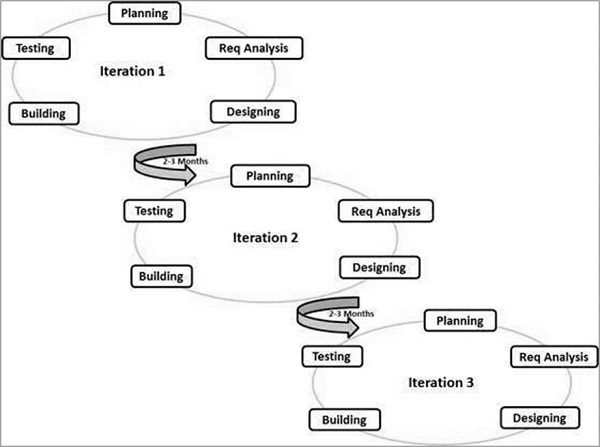
\includegraphics[scale=0.5]{images/AgileModel.jpg}
\caption{Agile Model}
\end{figure}


%\newpage

%\chapter{Technologies Used}
%
\section{Introduction to PHP}
\begin{figure}[h]
\centering \includegraphics[scale=0.4]{images/php.png}
\caption{Php logo}
\end{figure}
\noindent PHP is an open source server-side scripting language designed for Web development to produce dynamic Web pages. It is one of the first developed server-side scripting languages to be embedded into an HTML source document rather than calling an external file to process data. The code is interpreted by a Web server with a PHP processor module which generates the resulting Web page. It also has evolved to include a command-line interface capability and can be used in standalone graphical applications.\\

\noindent PHP can be deployed on most Web servers and also as a standalone shell on almost every operating system and platform, free of charge. A competitor to Microsoft’s Active Server Pages (ASP) server-side script engine and similar languages, PHP is installed on more than 20 million Web sites and 1 million Web servers. Notable software that uses PHP includes Drupal, Joomla, MediaWiki, and WordPress. PHP is a general-purpose scripting language.\\

\noindent It is especially suited to server-side web development where PHP generally runs on a web server. Any PHP code in a requested file is executed by the PHP runtime, usually to create dynamic web page content or dynamic images used on Web sites or elsewhere. It can also be used for command-line scripting and client-side graphical user interface (GUI) applications. PHP can be deployed on most Web servers, many operating systems.
\subsection{Features of PHP}
\begin{itemize}
\item Http Authentication
\item Cookies and Sessions
\item Connection Handling
\item Designer-friendly 
\item Cross platform Compatibility 
\item Loosely typed Language
\item Open Source
\item Easy code
\end{itemize}



\section{MySQL Database Server}
\begin{figure}[h]
\centering \includegraphics[scale=0.2]{images/mysql.jpg}
\caption{Mysql logo}
\end{figure}
\noindent I used the Mysql database for my project. It is world''s most popular open source database It 
is a relational database management system (RDBMS) that runs as a server 
providing multi-user access to a number of databases. It is named after 
developer Michael Widenius's daughter, My. The SQL phrase stands for
Structured Query Language. MySQL is written in C and C++.\\

\noindent Free-software-open source projects that require a 
full-featured database management system
often use MySQL. MySQL is also used in many high-profile, large-scale World 
Wide Web products, including
Wikipedia, Google (though not for searches) and Facebook.\\

\noindent MySQL is a popular choice of database for use in web 
applications, and is a central component of the widely used LAMP web 
application software LAMP is an acronym for “Linux, Apache, MySQL, 
Perl/PHP/Python”. MySQL is used in some of the most frequently visited web sites 
on the Internet, including Flickr, Nokia.com, YouTube, Wikipedia, Google 
and Facebook.\\

\noindent One of the greatest advantage of Django is that it synchronises the 
database only with one command withouut having any need to send 
different queries for insertion, deletion, updation etc. There is a 
file named models.py which is used for purpose of creating database.
\subsection{Features of MySQL}
\begin{itemize}
\item MySQL is a database management system.
\item MySQL is a relational database management system.
\item MySQL software is Open Source.
\item The MySQL Database Server is very fast, reliable, and easy to 
use.
\item MySQL Server works in client/server or embedded systems.
\item A large amount of contributed MySQL software is available.
\end{itemize}
\subsection{Installation of MySQL}
MySql can be installed using following commands:\\

\hspace{4pt} \$ sudo apt-get install mysql-server\\

\hspace{4pt} \$ sudo apt-get install mysql-client


\section{Introduction to Bootstrap} 

\begin{figure}[h]
\centering \includegraphics[scale=0.3]{images/bootstrap.png}
\caption{Bootstrap logo}
\end{figure}
\subsection{What is Bootstrap}
\noindent Bootstrap is a powerful front-end framework for faster and easier web development. It includes HTML and CSS based design templates for common user interface components like Typography, Forms, Buttons, Tables, Navigations, Dropdowns, Alerts, Modals, Tabs, Accordion, Carousel and many other as well as optional JavaScript extensions.
Bootstrap also gives you ability to create responsive layout with much less efforts.
\subsection{Advantages of Bootstrap}
The biggest advantage of using Bootstrap is that it comes with free set of tools for creating flexible and responsive web layouts as well as common interface components.
Additionally, using the Bootstrap data APIs you can create advanced interface components like Scrollspy and Typeaheads without writing a single line of JavaScript.
Here are some more advantages, why one should opt for Bootstrap:
\begin{itemize}
\item Save lots of time.
\item Responsive features.
\item Consistent design .
\item Easy to use.
\item Compatible with browsers.
\item Open Source.
\item Consistency.
\item Comprehensive List Of Components
\item Leveraging Javascript Libraries.
\item Frequent Updates.
\end{itemize}
\subsection{Installation of Bootstrap}
Downloading of Bootstrap is a very easy proccess.
Type the commands in the terminal:\\

 \$ git clone https://github.com/twbs/bootstrap.git\\


\noindent This will clone the bootstrap files on your pc/laptop and later u can use these files in your project.


\section{Introduction to Apache Web Server}

\begin{figure}[h]
\centering\includegraphics[scale=0.5]{images/apache.jpg}
\caption{Apache logo}
\end{figure}
\noindent Apache is a web server software notable for playing a key role in the initial 
growth of the World Wide Web. Apache is developed and maintained by an 
open community of developers under the auspices of the Apache Software 
Foundation. The application is available for a wide variety of operating 
systems, including Unix, FreeBSD, Linux, Solaris, Novell NetWare, Mac OS X, 
Microsoft Windows, OS/2, TPF, and eComStation. Released under the Apache 
License, Apache is open-source software.

\noindent The goal of this project is to provide a secure, efficient and extensible 
server that provides HTTP services in sync with the current HTTP standards.
\subsection{Features of Apache Server}
\begin{itemize}
\item Apache supports a variety of features, many implemented as compiled 
modules which extend the core functionality. These can range from 
server-side programming language support to authentication schemes. 
\item Apache features configurable error messages, DBMS-based 
authentication databases, and content negotiation. It is also supported 
by several graphical user interfaces (GUIs).
\item It supports password authentication and digital certificate 
authentication. Apache has a built in search engine and an HTML authorizing 
tool and supports FTP.
\end{itemize}

\subsection{Installation of Apache Server}
Apache web server can be installed using following commands:\\

\hspace{4pt} \$ sudo apt-get install apache2




%\section{Debconf}
%\input {input/debconf.tex}


\section{Introduction to Doxygen}
\input {input/doxygen.tex}


%\chapter{Experimental Results}
%\noindent Automated Building Drawings System is used to eliminate the previous manual process of creation of drawings using the traditional techniques by replacing it with the automated system, such that the end user can now easily make the required drawing design 
and the whole process can be made more easy and reliable for the users thus saving time. All the drawings can also be exported in some supported file format using this software thus making the system more useful and reliable.\\

\noindent User can easily maintain all the record of the previously created drawing designs by saving them into the computer memory. It eliminates the manual operations and thus
increases productivity in the system by automating it. Entities can be crated just by giving their names and parameters thus the whole process becomes a very fast. The Drawing can be easily generated for a particular building by giving all the specifications such as length of the walls, height, width etc thus managing the system overall. \\

\noindent Firstly the user input the required specifications of the desired design such as length, height, the type of entity etc. Then these parameters and all other details are saved in a input file which is a txt file. Then this file is parsed into the system where the processing is done and the input file is splitted into the output file where its parameters are separated into the lines. \\

\noindent This file then parsed into the system from which the system reads the content that is specified by the user and then according to that information the Automated Building Drawings system produces a drawing which can be opened using the cad software LibreCad.\\

\noindent The traditional pencil and paper work can be reduced to a great extent by doing work using this software and saving paper thus
making it environment friendly. Thus, making it automated process. Lot of time was wasted during the drawing of buildings using the pencil and paper. So with this software even the  people who is not proficient in computer can easily take the benefit of cration of drawings using this software.


\section{Testing}
The most important activity at the implementation stage is the system testing with the objective of validating the system against the designed criteria. During the development cycle, user was involved in all the phases that are analysis, design and coding. After each phase the user was asked whether he was satisfied with the output and the desired rectification was done at the moment. During coding, generally bottom up technique is used. Firstly the lower level modules are coded and then they are integrated together.

Software testing is an investigation conducted to provide stakeholders with information about the quality of the product or service under test.Software testing can also provide an objective, independent view of the software to allow the business to appreciate and understand the risks of software implementation. Test techniques include the process of executing a program or application with the intent of finding software bugs (errors or other defects). Software testing involves the execution of a software component or system component to evaluate one or more properties of interest. In general, these properties indicate the extent to which the component or system under test:
\begin{itemize}
	\item meets the requirements that guided its design and development,
	\item responds correctly to all kinds of inputs,
	\item performs its functions within an acceptable time,
	is sufficiently usable,
	\item can be installed and run in its intended environments, and achieves the general result its stakeholders desire.
\end{itemize}

As the number of possible tests for even simple software components is practically infinite, all software testing uses some strategy to select tests that are feasible for the available time and resources. As a result, software testing typically (but not exclusively) attempts to execute a program or application with the intent of finding software bugs (errors or other defects). The job of testing is an iterative process as when one bug is fixed, it can illuminate other, deeper bugs, or can even create new ones.

Software testing can provide objective, independent information about the quality of software and risk of its failure to users and/or sponsors.
Software testing can be conducted as soon as executable software (even if partially complete) exists. The overall approach to software development often determines when and how testing is conducted. For example, in a phased process, most testing occurs after system requirements have been defined and then implemented in testable programs. In contrast, under an Agile approach, requirements, programming, and testing are often done concurrently.

Thus before implementation, it involves the testing of the system. The testing phase involves testing first of separate parts of the system and then finally of the system as a whole. Each independent module is tested first and then the complete system is tested. This is the most important phase of the system development. The user carries out this testing and test data is also prepared by the user to check for all possible combinations of correct data as well as the wrong data that is trapped by the system. So the testing phase consists of the following steps:

\subsection{Unit Testing}
In the bottom of coding technique, each module is tested individually. Firstly the module is tested with some test data that covers all the possible paths and then the actual data was fed to check for results.Unit testing, also known as component testing, refers to tests that verify the functionality of a specific section of code, usually at the function level. In an object-oriented environment, this is usually at the class level, and the minimal unit tests include the constructors and destructors.

These types of tests are usually written by developers as they work on code (white-box style), to ensure that the specific function is working as expected. One function might have multiple tests, to catchcorner cases or other branches in the code. Unit testing alone cannot verify the functionality of a piece of software, but rather is used to ensure that the building blocks of the software work independently from each other.

Unit testing is a software development process that involves synchronized application of a broad spectrum of defect prevention and detection strategies in order to reduce software development risks, time, and costs. It is performed by the software developer or engineer during the construction phase of the software development lifecycle. Rather than replace traditional QA focuses, it augments it. Unit testing aims to eliminateconstruction errors before code is promoted to QA; this strategy is intended to increase the quality of the resulting software as well as the efficiency of the overall development and QA process.

Depending on the organization's expectations for software development, unit testing might include static code analysis, data-flow analysis, metrics analysis, peer code reviews, code coverage analysis and other software verification practices.

\subsection{Integration Testing}
After all the modules are ready and duly tested, these have to be integrated into the application. This integrated application was again tested first with the test data and then with the actual data.

Integration testing is any type of software testing that seeks to verify the interfaces between components against a software design. Software components may be integrated in an iterative way or all together ("big bang"). Normally the former is considered a better practice since it allows interface issues to be located more quickly and fixed.

Integration testing, also known as integration and testing (I\&T), is a softwaredevelopment process which program units are combined and tested as groups in multiple ways. In this context, a unit is defined as the smallest testable part of anapplication. Integration testing can expose problems with the interfaces among program components before trouble occurs in real-world program execution. Integration testing is a component of Extreme Programming (XP), a pragmatic method of software development that takes a meticulous approach to building a product by means of continual testing and revision.
Once all the individual units are created and tested, we start combining those “Unit Tested” modules and start doing the integrated testing. So the meaning of Integration testing is quite straight forward- Integrate/combine the unit tested module one by one and test the behaviour as a combined unit.

The main function or goal of Integration testing is to test the interfaces between the units/modules.
The individual modules are first tested in isolation. Once the modules are unit tested, they are integrated one by one, till all the modules are integrated, to check the combinational behavior, and validate whether the requirements are implemented correctly or not.
Here we should understand that, Integration testing does not happens at the end of the cycle, rather it is conducted simultaneously with the development. So in most of the times all the modules are not actually available to test and here is what the challenge comes to test something which does not exists!

Integration testing works to expose defects in the interfaces and interaction between integrated components (modules). Progressively larger groups of tested software components corresponding to elements of the architectural design are integrated and tested until the software works as a system.

\subsection{Parallel Testing}
The third in the series of tests before handling over the system to the user is the parallel processing of the old and the new system. At this stage, complete and thorough testing is done and supports out the event that goes wrong. This provides the better practical support to the persons using the system for the first time who may be uncertain or even nervous using it.

Parallel testing is a testing technique in which the same inputs are entered in two different versions of the application and reporting the anomalies. Since the system that is being tested will be the new means by which payroll is calculated, parallel testing should be managed by those who will be regularly taking care of payroll responsibilities. This allows hands-on training and generates invaluable troubleshooting experience before the system even goes live. Unfortunately, this usually doubles the workload for these employees that have to enter payroll information into both the new and old system, so additional help may be needed during this transition phase. When needed, managers within the organization that have more experience with the new system or vendor representatives may help to answer questions and provide information.

Executing test runs in parallel is obviously very important if many test runs need to be executed. The goal is to exploit the available resources as well as possible. If several machines are available, the goal is to achieve linear speedup; that is, the running time of executing all tests decreases linearly with the number of machines. In order to achieve this speed-up, it is important to balance the load on all machines – just as in all parallel applications .At the same time, however, it is also important to control the state of the test database(s) and to execute the test runs in such a way that the number of database reset operations is minimized – just as for non-parallel testing in .As a result, parallel testing involves solving a two-dimensional optimization problem: (a) partitioning: deciding which test runs to execute on which machine; and (b) ordering: deciding in which order to execute the test runs on each machine.

Parallel testing is a two dimensional scheduling problem. In addition to deciding in which order to execute the test runs, a scheduling strategy must partition the test runs. Depending on the architecture, Shared-Database or Shared-Nothing (see below), a parallel execution can increase the number of resets due to interference (Shared-Database) or decrease the number of resets (Shared-Nothing) by executing test runs that are in conflict concurrently. As a result, conflict information ought to be taken into account in order to decide on which machine to execute which test run. 

Furthermore, it is important to balance the load on all machines so that the resources are used as well as possible. Load balancing can be carried out without conflict information; load balancing should be carried out taking the current load of machines and the estimated length of test runs into account.

\chapter{System Design}

\section{Object Oriented}

Object-oriented design is the process of planning a system of interacting objects for the purpose of solving a software problem. It is one approach to software design. An object contains encapsulated data and procedures grouped together to represent an entity. The 'object interface' defines how the object can be interacted with. An object-oriented program is described by the interaction of these objects. Object-oriented design is the discipline of defining the objects and their interactions to solve a problem that was identified and documented during object-oriented analysis.

\iffalse
 basic requirement of this app is that the user must be having ANDROID
Operating System in his phone or tablet. The minimum version of Androids Operating
System must be ICECREAM SANDWICH. All the versions of Android OS above
IcecreamSandwich( i.e. Jellybean, Kitkat, Lollipop,Marshmallows) will support this
app. A user needs Monitary app installed in device .


\noindent As shown in the Figure \ref{fig:1}, .\\Brief introduction showing the features available in the application.

\begin{figure}[ht]
\centering
\includegraphics[scale=0.5]{images/s1.png}
\caption{Screen 1}
\label{fig:1}
\end{figure}

\noindent This are the options the navigation drawer the app will contain. These will contain the screens the user can navigate too that can be seen in Figure \ref{fig:2}. \\

\begin{figure}[ht]
	\centering
	\includegraphics[scale=0.49]{images/s2.png}
	\caption{Screen 2}
	\label{fig:2}
\end{figure}

\noindent  Statistics will be able to change according to the dates selected. Default values will be the current week. User Will be able to see diagrams according to Quantity and
days, Quantity and categories and others.as seen in the Figure \ref{fig:3}.\\

\begin{figure}[ht]
\centering
\includegraphics[scale=0.5]{images/s3.png}
\caption{Screen 3}
\label{fig:3}
\end{figure}

\noindent Reminder view will contain details from the reminder created and the user can edit
the reminder values. in Figure \ref{fig:4}. \\

\begin{figure}[ht]
\centering
\includegraphics[scale=0.38]{images/s4.png}
\caption{Screen 4}
\label{fig:4}
\end{figure}

\noindent Reminder screen will show the current saved Reminder and if they are active or not.
To activate one it will have a switch next to the name so it can be activated in any
moment. The user will be able to erase and add from this view as seen in the Figure \ref{fig:5}. It's named as output.dxf. We can open that file in LibreCAD directly from the command-line.\\


\begin{figure}[ht]
\centering
\includegraphics[scale=0.5]{images/s6.png}
\caption{Screen 5}
\label{fig:5}
\end{figure}

\noindent Expenses View is the main screen that will be showed. The user will be able to add expenses and see a total amount in Today, Week and Month. as shown in Figure \ref{fig:6}. 

\begin{figure}[ht]
\centering
\includegraphics[scale=0.38]{images/s61.png}
\caption{Screen 6}
\label{fig:6}
\end{figure}

\noindent This activity will provide necessary help to the user. One can also mail the maker
(GURNOOR SINGH) for further queries as shown in Figure \ref{fig:7}. 

\begin{figure}[ht]
\centering
\includegraphics[scale=0.38]{images/s7.png}
\caption{Screen 7}
\label{fig:7}
\end{figure}
\noindent User will be able to add and delete categories from the Categories View \ref{fig:8}. 

\begin{figure}[ht]
\centering
\includegraphics[scale=0.38]{images/s8.png}
\caption{Screen 8}
\label{fig:8}
\end{figure}
\fi

\section{Detail Design}

	\subsection{Registration}
	When the user first launches the app he sees the splash screen, if he is not logged in then he will see the login screen, if he hasn't created any account yet then he will have to register first, After submitting details during registration he will recieve an email confirming his email account. On successful email confirmation, he can login in the app. \\
	
	\subsection{Home}
	After Successful login, he will see the home screen, which will be the introduction page of sports department.After that user will have access to the following parts : 
	\begin{itemize}
		\item \textbf{Bottom Slider}:- This part is available in the admin panel application.Under this feature admin has access to add news related to athlatic meet, sports day or any latest information added to the department.Admin also has access to add achievement of students in sports. 
				
		\item \textbf{Navigation Drawer Menu}:- It is the main menu of the app. It opens by left swiping. It contains following options:
		\begin{itemize}
			\item \textbf{Introduction}:- It will give introduction about the sports department.Mission and Vision is also discussed under this pannel.
			
			\item \textbf{Commitee}:- It shows the list of commitee members currently available in the sports department.
			
			\item \textbf{Latest News}:- Here admin can upload the latest news about of the sports department. Admin can also upload image if required with the news.
			
			\item \textbf{Facilities}:-It shows the facilities that sports department of college provide to their students such as gym , cricket groung etc.
			
			\item \textbf{Athletic Meet}:- By Clicking this user will get latest news about athletic meet , results of the athletic meet and also the records made under meet.
			
			\item \textbf{Scholarship}:It shows the scholarships currently available in the college for sports department.
			
			\item \textbf{Analysis}:-It will display the anaylsis part of the participation engineering branches made in a particular year.
			
			\item \textbf{Achievement}:-It will have two options:
			\begin{itemize} 
			\item \textbf{Intramural}:-Achievement of students who participated or got medals in activities or events performed under college boundaries will be displayed here.
			\item \textbf{Extramural}:-Achievement of students who participated or got medals in activities or events performed outside of college boundaries will be displayed here.
			\end{itemize}
			\item \textbf{Communicate}:-
			\begin{itemize} 
			\item \textbf{Contact Us}:-It will display the contacts of sports department.Also Email-Id will be thier of sports department. 
			\item \textbf{Map}:-It will display the map of sports department.
\item \textbf{Share}:-It will help the user to share the application with another member.User can share the application in whatsapp , facebook , messanger etc.
\item \textbf{Developers}:-It will display the information of the developers who developed GNDEC Sports.  			
			
			\end{itemize}
			
		\end{itemize}
	\end{itemize}

\section{System Design}

\newpage
\begin{figure}[ht]
	
	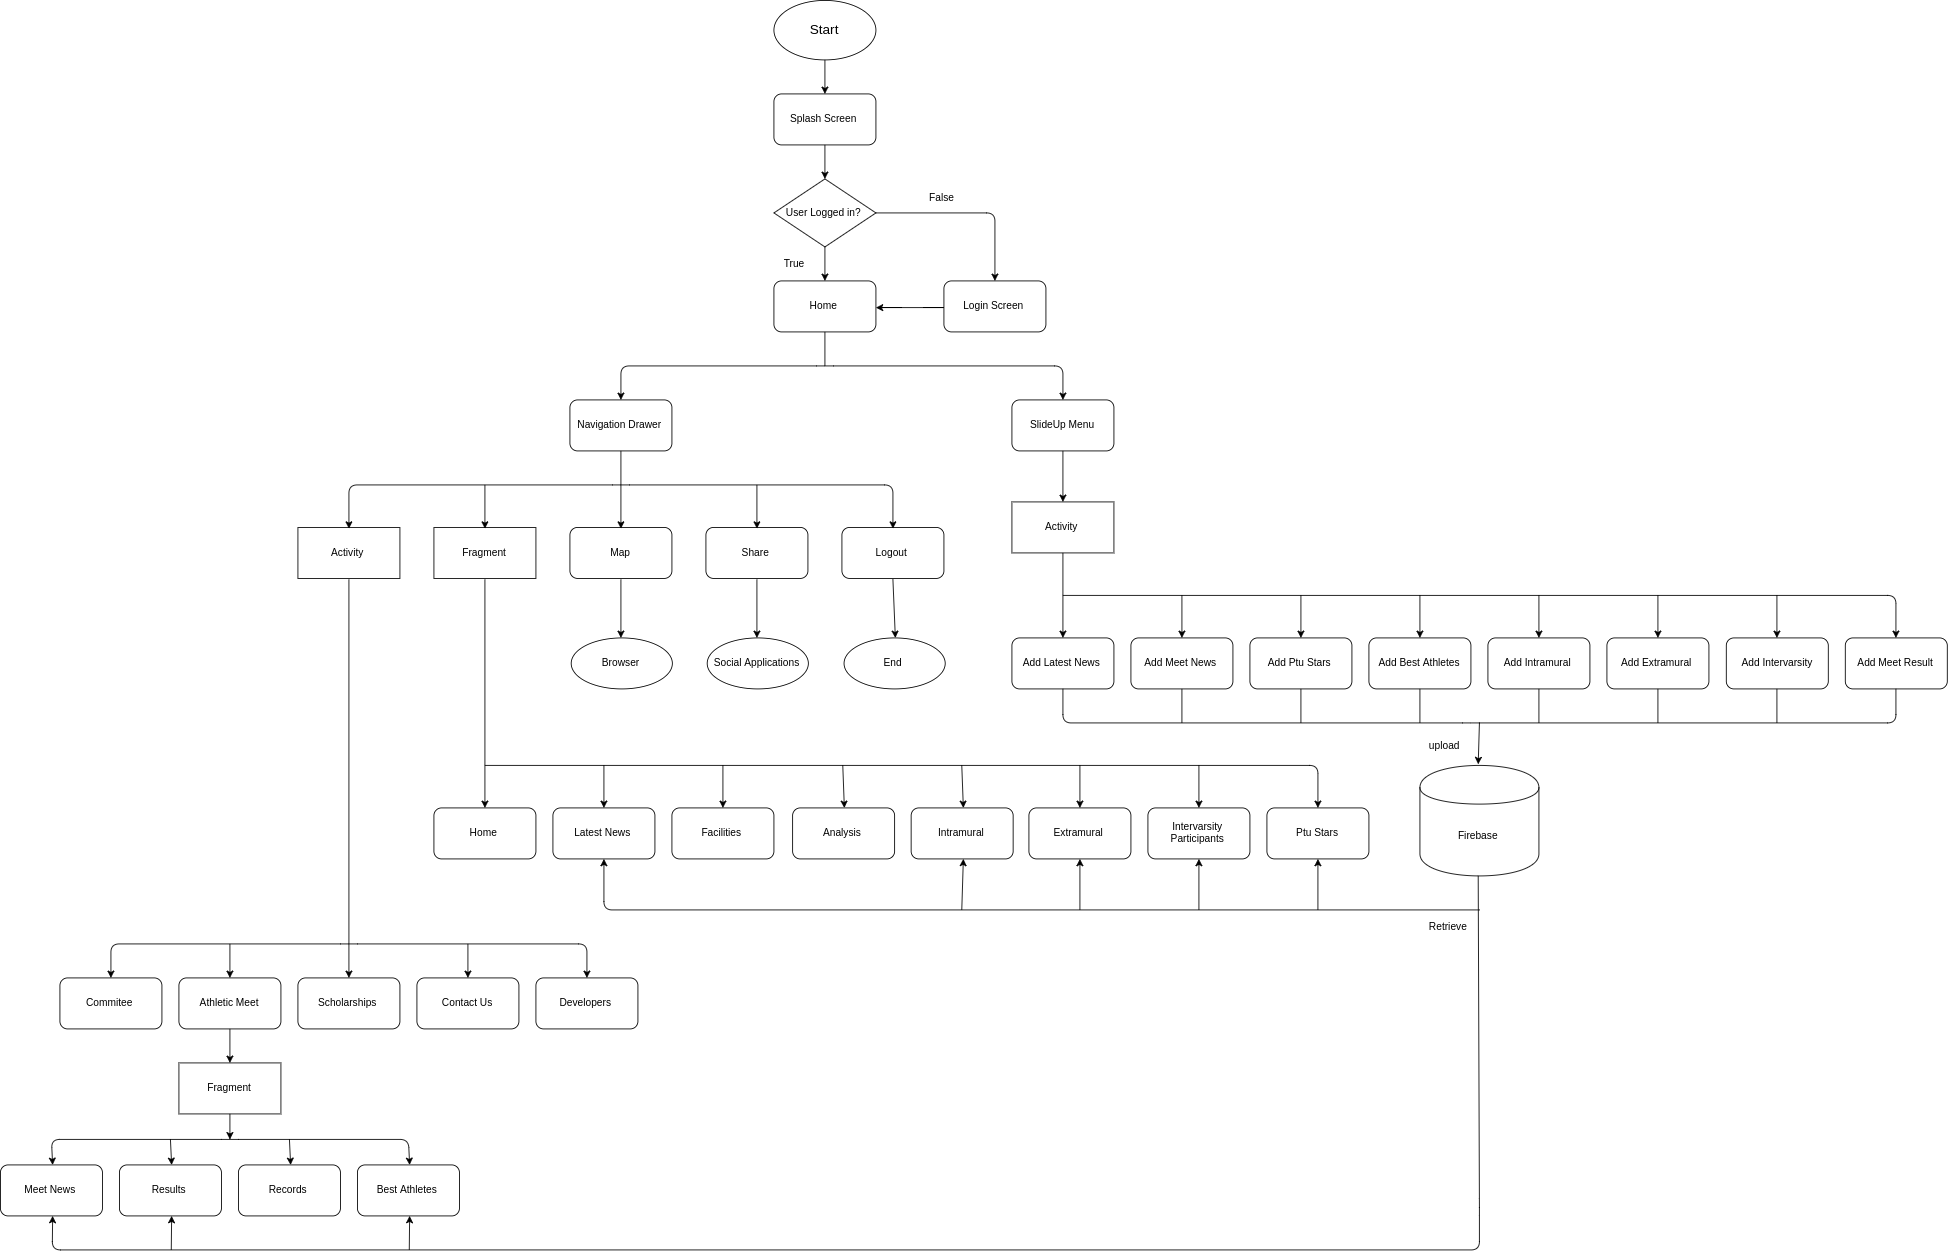
\includegraphics[scale=0.25]{images/Gndecadmingne.png}
	\caption{Flow Chart of gndec admin}
\end{figure}

\newpage
\begin{figure}[ht]
	
	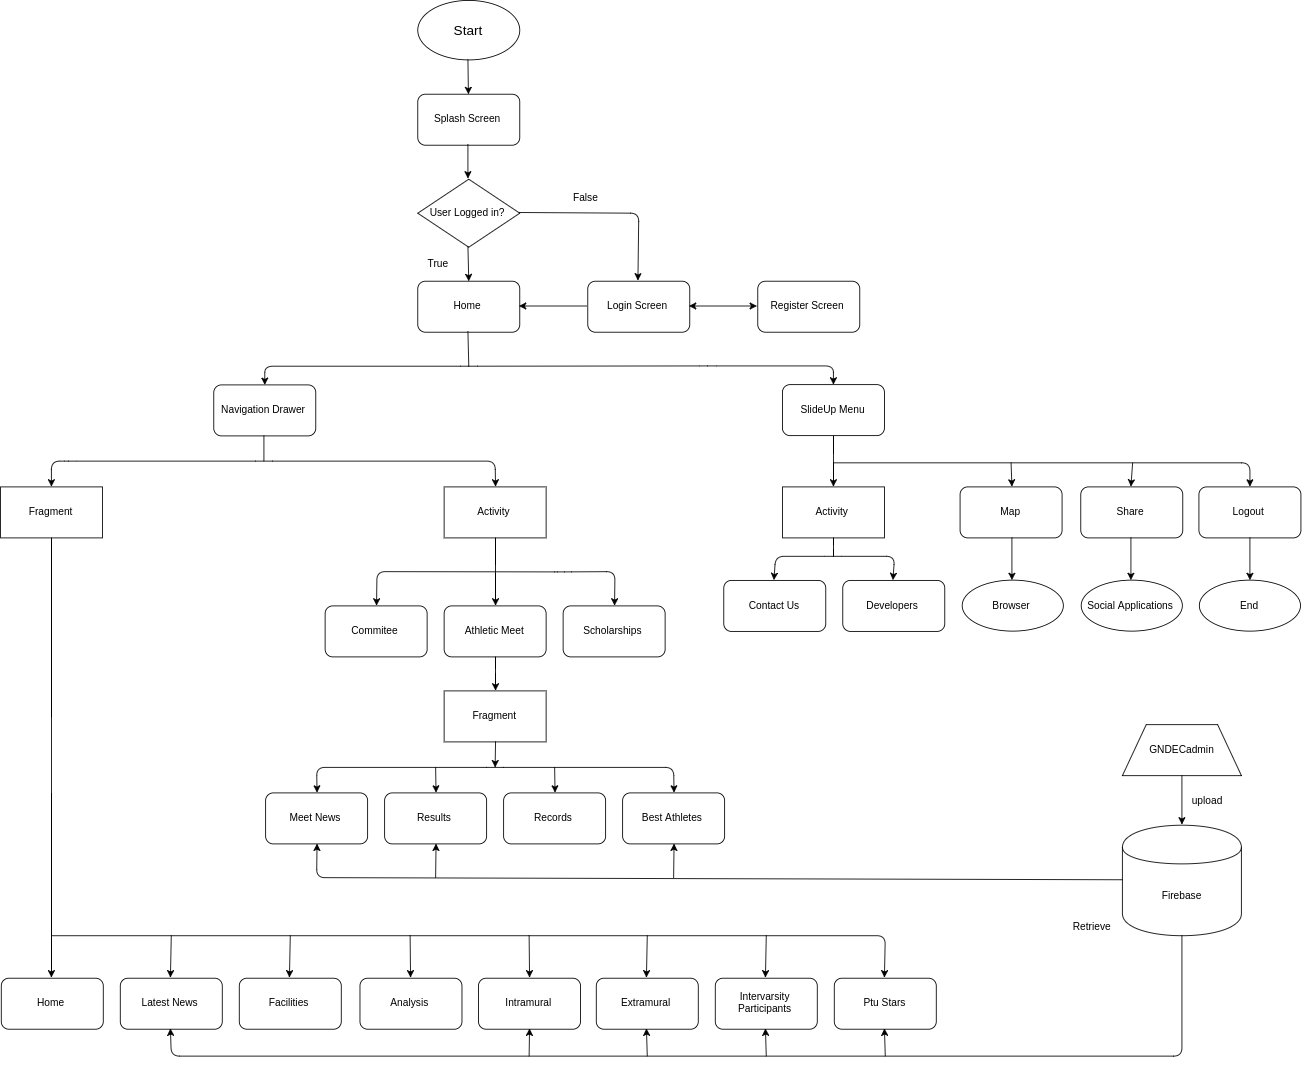
\includegraphics[scale=0.35]{images/Gndecstudent.png}
	\caption{Flow Chart of gndec student}
\end{figure}




\section{Database Design}

\newpage	
	\begin{figure}[ht]
		\centering
		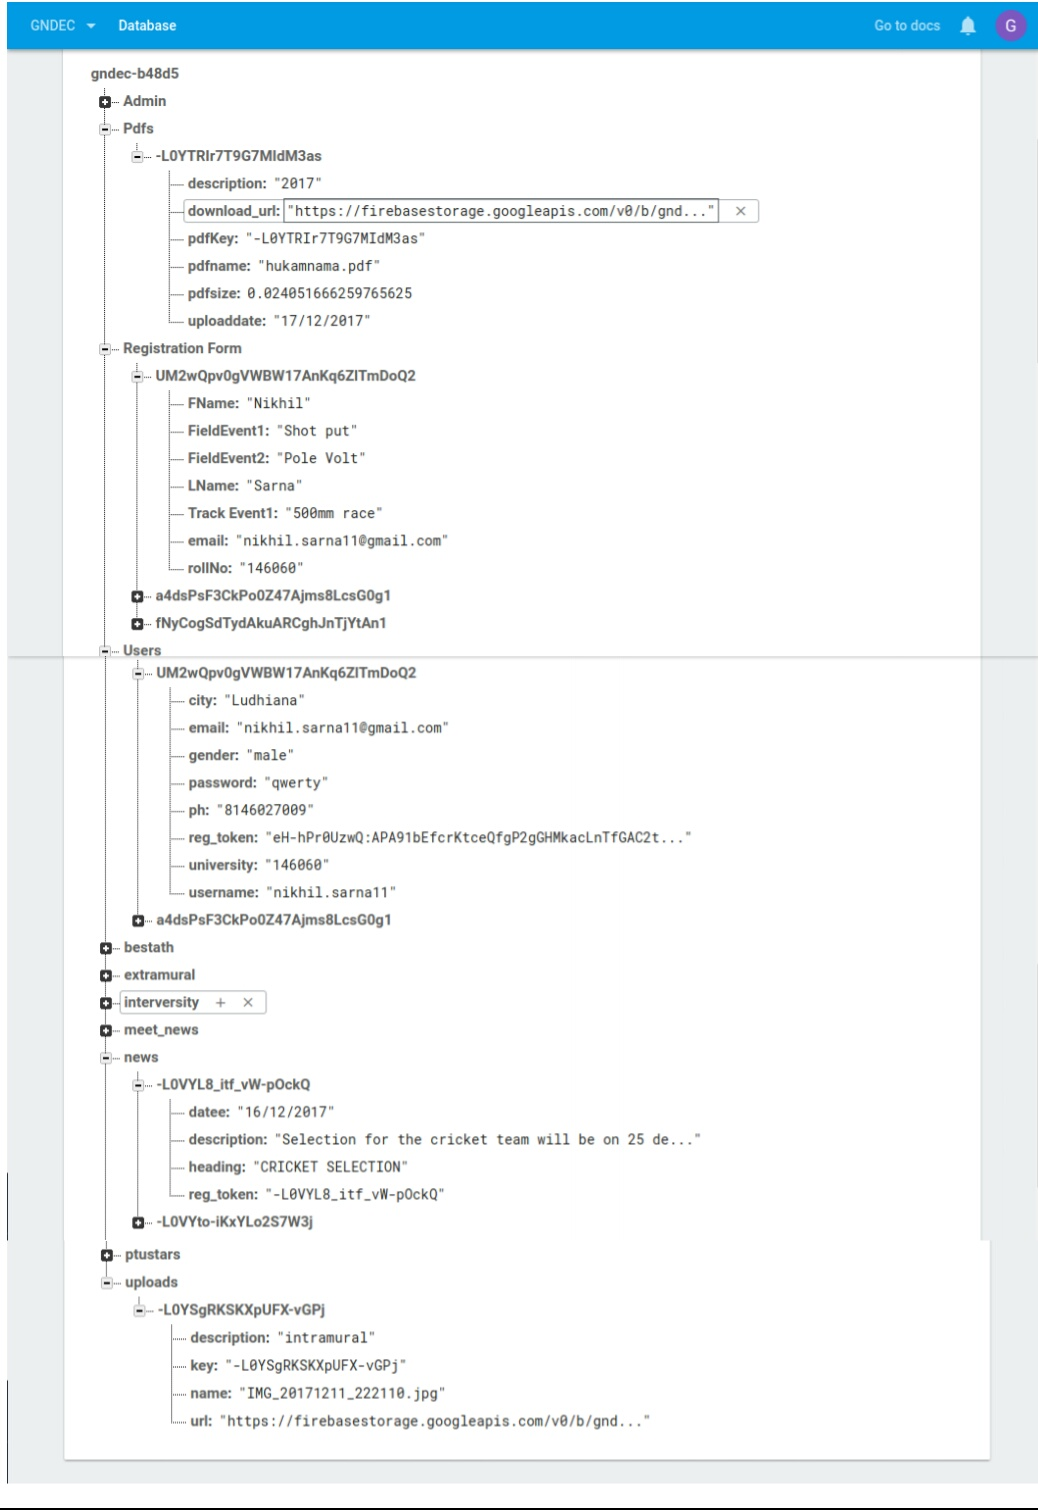
\includegraphics[scale=0.20]{images/dbfire.jpg}
		\caption{ER Diagram}
	\end{figure}

	\subsection{ER Diagram}
	
\newpage	
	\begin{figure}[ht]
		\centering
		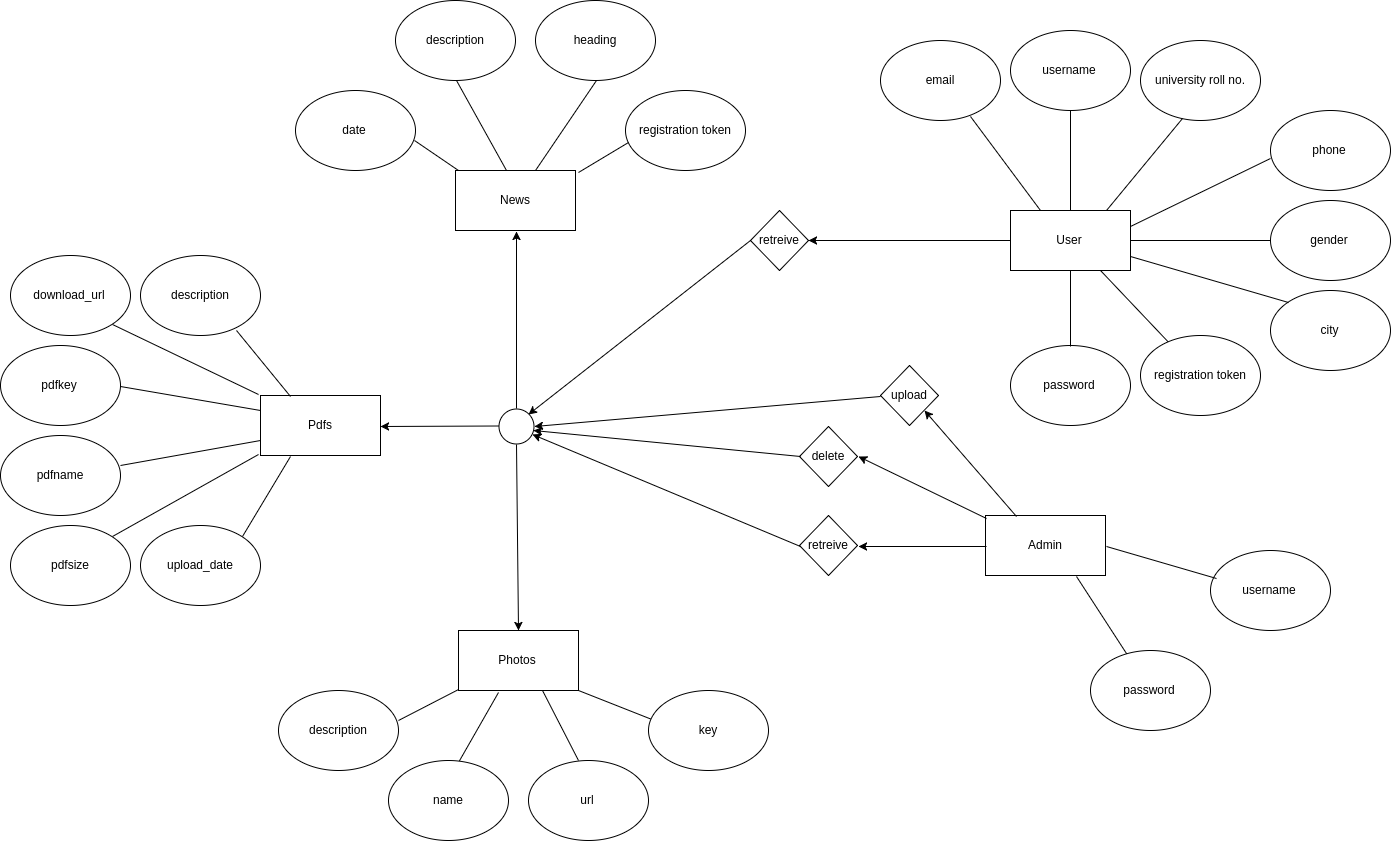
\includegraphics[scale=0.35]{images/ergndec.png}
		\caption{ER Diagram}
	\end{figure}
	
	\subsection{Database Connection Controls and Strings}
	The Firebase Realtime Database is a cloud-hosted database. Data is stored as JSON and synchronized in realtime to every connected client. When we build cross-platform apps with our iOS, Android, and JavaScript SDKs, all of our clients share one Realtime Database instance and automatically receive updates with the newest data. \\
	
	If we are using the latest version of Android Studio (version 2.2 or later), It is recommended using the Firebase Assistant to connect your app to Firebase. The Firebase Assistant can connect our existing project or create a new one for us and automatically install any necessary gradle dependencies.\\
	
	If we are using an older version of Android Studio or have a more complex project configuration, we can still manually add Firebase to our app.
	
		\subsubsection{Using the Firebase Assistant}
		
		To open the Firebase Assistant in Android Studio:
		\begin{itemize}
			\item Click Tools > Firebase to open the Assistant window.
			\item Click to expand one of the listed features (for example, Analytics), then click the provided tutorial link (for example, Log an Analytics event).
			\item Click the Connect to Firebase button to connect to Firebase and add the necessary code to your app.
		\end{itemize}
	
		\subsubsection{Manually adding Firebase}
		To add Firebase to your app you'll need a Firebase project and a Firebase configuration file for your app.
		\begin{itemize}
			\item Create a Firebase project in the Firebase console, if we don't already have one. If we already have an existing Google project associated with our mobile app, click Import Google Project. Otherwise, click Add project.
			\item Click Add Firebase to our Android app and follow the setup steps. If we're importing an existing Google project, this may happen automatically and we can just download the config file.
			\item When prompted, enter our app's package name. It's important to enter the package name our app is using, this can only be set when we add an app to our Firebase project.
			\item At the end, we'll download a google-services.json file. We can download this file again at any time.
		\end{itemize}



\chapter{Implementation ,Testing and Maintenance}
\section{Introduction to Languages,IDE’s,Tools and Technologies used for Implementation}
	
\subsection{Technologies used}

\subsubsection{Firebase}

Firebase helps you build better mobile apps and grow your business.

Firebase is a mobile platform from Google offering a number of different features that you can pick ‘n mix from. Specifically, these features revolve around cloud services, allowing users to save and retrieve data to be accessed from any device or browser. This can be useful for such things as cloud messaging, hosting, crash reporting, notifications, analytics and even earning money through AdMob.

It works with Android apps, iOS apps and web apps and best of all: it’s free!

\begin{itemize}

\item \textbf{Setting up a project}

Before you can do anything with Firebase, you first need to create an account. You can do this over at firebase.google.com.

\begin{figure}[ht]
\centering
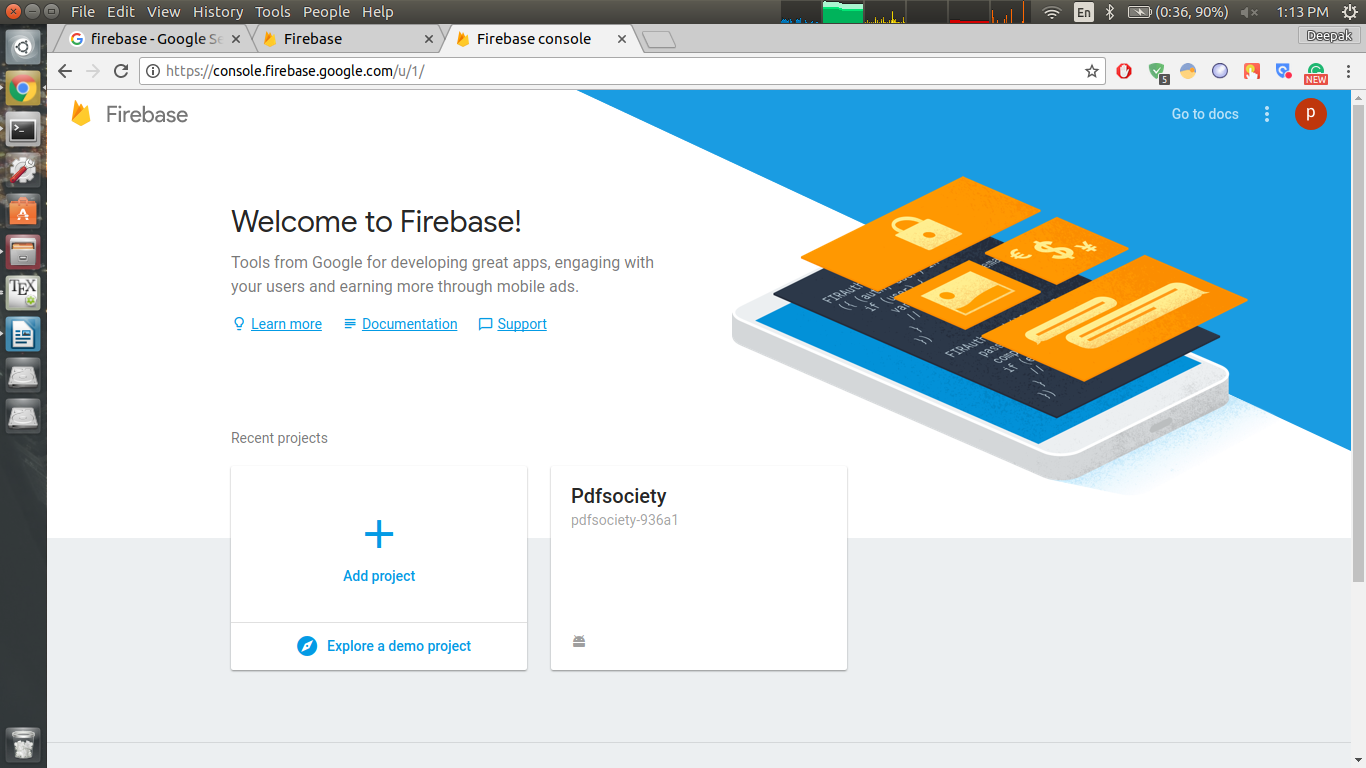
\includegraphics[scale=0.20]{images/Pdf2.png}
\caption{Firebase Console}
\end{figure}

 

\item \textbf{Firebase Products}

\begin{figure}[ht]
\centering
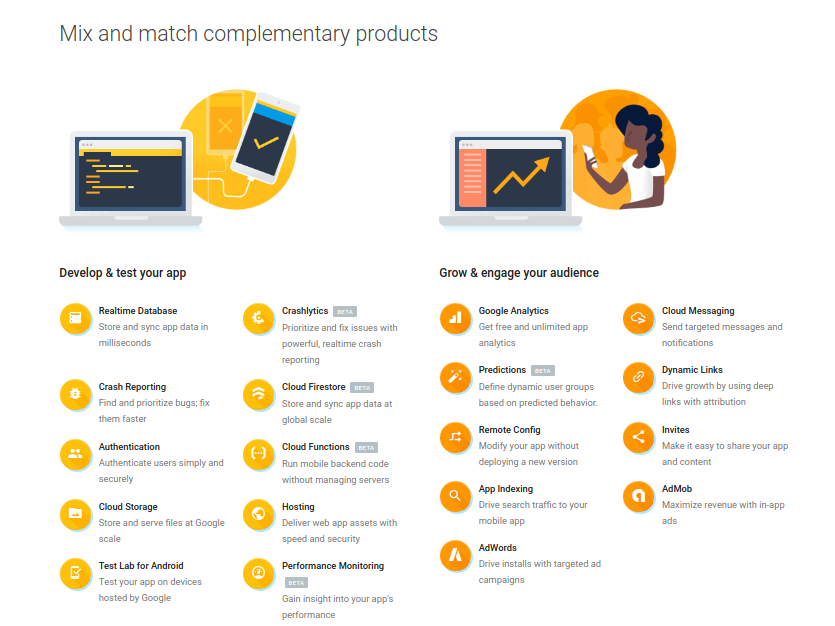
\includegraphics[scale=0.4]{images/Pdf1.png}
\caption{Firebase Products}
\end{figure}

\begin{itemize}

\item \textbf{Firebase Authentication}

Firebase Authentication aims to make building secure authentication systems easy, while improving the sign-in and onboarding experience for end users. It provides an end-to-end identity solution, supporting email and password accounts, phone auth, and Google, Twitter, Facebook, and GitHub login, and more.

Most apps need to know the identity of a user. Knowing a user's identity allows an app to securely save user data in the cloud and provide the same personalized experience across all of the user's devices.
Firebase Authentication provides backend services, easy-to-use SDKs, and ready-made UI libraries to authenticate users to your app. It supports authentication using passwords, phone numbers, popular federated identity providers like Google, Facebook and Twitter, and more.

Firebase Authentication integrates tightly with other Firebase services, and it leverages industry standards like OAuth 2.0 and OpenID Connect, so it can be easily integrated with your custom backend.

\item \textbf{Firebase Realtime Database}

Store and sync data with our NoSQL cloud database. Data is synced across all clients in realtime, and remains available when your app goes offline.

The Firebase Realtime Database is a cloud-hosted database. Data is stored as JSON and synchronized in realtime to every connected client. When you build cross-platform apps with our iOS, Android, and JavaScript SDKs, all of your clients share one Realtime Database instance and automatically receive updates with the newest data.


\item \textbf{Cloud Storage}

Cloud Storage is built for app developers who need to store and serve user-generated content, such as photos or videos.

Cloud Storage for Firebase is a powerful, simple, and cost-effective object storage service built for Google scale. The Firebase SDKs for Cloud Storage add Google security to file uploads and downloads for your Firebase apps, regardless of network quality. You can use our SDKs to store images, audio, video, or other user-generated content. On the server, you can use Google Cloud Storage, to access the same files.
	\end{itemize}
	\end{itemize}
	
\subsubsection{Android}


Android provides a rich application framework that allows you to build innovative
apps and games for mobile devices in a Java language environment. The documents
listed in the left navigation provide details about how to build apps using Android's
various APIs.The various fundamental concepts about the Android app framework:

\begin{figure}[ht]
\centering
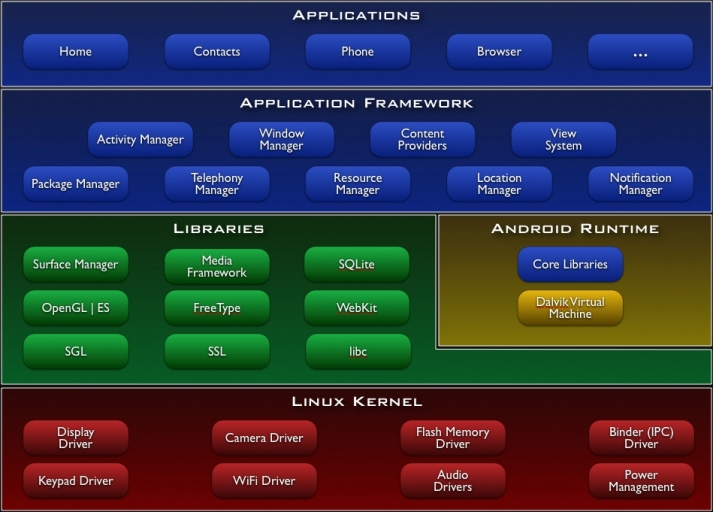
\includegraphics[scale=0.38]{images/a1.jpg}
\caption{Android Anatomy}
\label{fig:Anatomy}
\end{figure}

Apps provide multiple entry points.Android apps are built as a combination of distinct components that can be invoked individually. For instance, an individual activity provides a single screen for a userinterface, and a service independently performs work in the background. From one component you can start another component using an intent. You can even start a component in a different app, such as an activity in a maps app to show an
address. This model provides multiple entry points for a single app and allows any
app to behave as a user's "default" for an action that other apps may invoke.

Apps adapt to different devices, Android provides an adaptive app framework that allows you to provide unique resources for different device configurations. For example, you can create different XML layout les for different screen sizes and the system determines which layout
to apply based on the current device's screen size. You can query the availability of device features at runtime if any app features require specific hardware such as
a camera. If necessary, you can also declare features your app requires so app markets such as Google Play Store do not allow installation on devices that do not
support that feature Android comes with an Android market which is an online
software store. It was developed by Google.

 It allows Android users to select, and
download applications developed by third party developers and use them. There
are around 2.0 lack+ games, application and widgets available on the market for
users. Android applications are written in java programming language. Android is
available as open source for developers to develop applications which can be
further used for selling in android market. There are around 200000 applications
developed for android with over 3 billion+ downloads. Android relies on Linux version 2.6 for core system services such as security, memory management, process management, network stack, and driver model. For software development, Android provides Android SDK (Software development kit).

\begin{itemize}

\item \textbf{Activity Lifecycle}
Activities in the system are managed as an activity stack. When a new activity
is started, it is placed on the top of the stack and becomes the running activitythe previous activity always remains below it in the stack, and will not come to
the foreground again until the new activity exits. An activity has essentially four
states:
If an activity in the foreground of the screen (at the top of the stack), it is
active or running.

If an activity has lost focus but is still visible (that is, a new non-full-sized or
transparent activity has focus on top of your activity), it is paused. A paused
activity is completely alive (it maintains all state and member information and
remains attached to the window manager), but can be killed by the system in
extreme low memory situations.
\begin{figure}[ht]
\centering
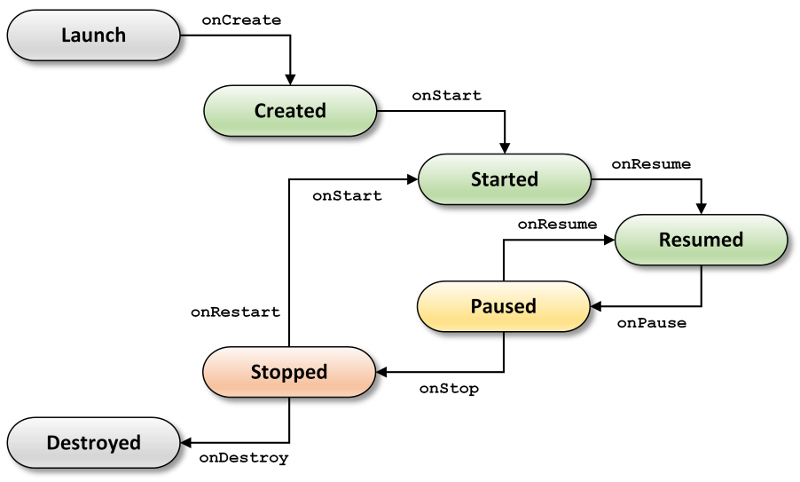
\includegraphics[scale=0.5]{images/a2.png}
\caption{Activity Life Cycle}
\label{fig: Activity }
\end{figure}

If an activity is completely obscured by another activity, it is stopped. It still
retains all state and member information, however, it is no longer visible to
the user so its window is hidden and it will often be killed by the system when
memory is needed elsewhere.

If an activity is paused or stopped, the system can drop the activity from memory by either asking it to finish, or simply killing its process. When it is displayed again to the user, it must be completely restarted and restored to its previous state.


\item \textbf{Libraries used in making this application}

\begin{itemize}
	\item \textbf{Android Support Library}
Android Support Library, Card View, Recycler View, Material : The application will
follow Material design guidelines.

\end{itemize}

\end{itemize}

\subsection{Language used}
\subsubsection{JAVA}

Java is a platform-independent programming language used to create secure
and robust application that may run on a single computer or may be distributed
among servers and clients over a network.

Java features such as platform-independency and portability ensure that while
de-veloping Java EE enterprise applications, you do not face the problems
related to hardware , network , and the operating system.

Java was started as a project called "Oak" by James Gosling in June 1991.
Gosling's goals were to implement a virtual machine and a language that had a
familiar C like notation but with greater uniformity and simplicity than C/C++.
The First publication of Java 1.0 was released by Sun Microsystems in 1995. It
made the promise of "Write Once, Run Anywhere", with free runtimes on
popular platforms. In 2006-2007 Sun released java as open source and
andplateform independent soft-ware. Over time new enhanced versions of Java
have been released. The current version of Java is Java 1.7 which is also
known as Java 7.he Java virtual machine (JVM) is a software implementation of
a computer that executes programs like a real machine. The Java virtual
machine is written specifically for a specific operating system, e.g. for Linux a
special implementation is required as well as for Windows.

Java programs are compiled by the Java compiler into bytecode. The Java
virtual machine interprets this bytecode and executes the Java program.
The Java runtime environment (JRE) consists of the JVM and the Java class li-
braries and contains the necessary functionality to start Java programs.
The JDK contains in addition the development tools necessary to create Java
pro-grams. The JDK consists therefore of a Java compiler, the Java virtual
machine, and the Java class libraries.

The characteristics and features of java are as follows :

\begin{itemize}
	\item \textbf{Simple}
Simple Java is a simple language because of its various features, Java
Doesn?t Support Pointers , Operator Overloading etc. It doesnt require
unreferenced object because java support automatic garbage collection.
Java provides bug free system due to the strong memory management.

\item \textbf{OOPS}
Object-Oriented Programming Language (OOPs) is the
methodology which provide software development and maintenance by
using
object
state,
behavior
Programming Lan-guage
must
,
and
have
properties.
the
Object Oriented following characteristics.
\begin{itemize}
	\item Encapsulation
\item Polymor-phism
 \item Inheritance
\item Abstraction

\end{itemize}
As the languages like Objective C, C++ fullls the above four characteristics yet
they are not fully object oriented lan-guages because they are structured
as well as object oriented languages.In java everything is an Object. Java
can be easily extended since it is based on the Object model.
\item \textbf{Secure}
Secure Java is Secure Language because of its many features it enables to
develop virus-free, tamper-free systems. Authentication techniques are
based on public-key encryption. Java does not support pointer explicitly for
the memory. All Program Run under the sandbox.

\item \textbf{Robust}
Robust Java was created as a strongly typed language. Data type issues
and problems are resolved at compile-time, and implicit casts of a variable
from one type to another are not allowed.
\item \textbf{Platform-independent}
Platform-independent Java Language is platform-independent due to its
hardware and software environment. Java code can be run on multiple
plat-forms e.g. windows, Linux, sun Solaris, Mac/Os etc. Java code is
compiled by the compiler and converted into byte code. This byte code is a
platform independent code because it can be run on multiple platforms i.e.
Write Once and Run Anywhere(WORA).
\item \textbf{Architectural Neural}
Architecture neutral It is not easy to write an application that can be used
on Windows , UNIX and a Macintosh. And its getting more complicated
with the move of windows to non Intel CPU architectures.
Java takes a diffierent approach. Because the Java compiler creates byte
code instructions that are subsequently interpreted by the java interpreter,
archi-tecture neutrality is achieved in the implementation of the java
interpreter for each new architecture.
\item \textbf{Portable}
Portable Java code is portable. It was an important design goal of Java that it
be portable so that as new architectures(due to hardware, operating system,
or both) are developed, the java environment could be ported to them.
In java, all primitive types(integers, longs, oats, doubles, and so on) are
20of de ned sizes, regardless of the machine or operating system on which
the program is run. This is in direct contrast to languages like C and C++
that leave the sized of primitive types up to the compiler and developer.
Additionally, Java is portable because the compiler itself is written in Java.
\item \textbf{Dynamic}
Dynamic Because it is interpreted , Java is an extremely dynamic language, At
runtime, the java environment can extends itself by linking in classes that may
be located on remote servers on a network(for example, the internet)
At runtime, the java interpreter performs name resolution while linking in the
necessary classes. The Java interpreter is also responsible for determining
the placement of object in memory. These two features of the Java interpreter
solve the problem of changing the de nition of a class used by other classes.
\item \textbf{Interpreted}
We all know that Java is an interpreted language as well. With
an interpreted language such as Java, programs run directly from the
source code.
The interpreter program reads the source code and translates it on the y
into computations. Thus, Java as an interpreted language depends on an
interpreter program.
The versatility of being platform independent makes Java to outshine from
other languages. The source code to be written and distributed is platform
independent.
Another advantage of Java as an interpreted language is its error
debugging quality. Due to this any error occurring in the program gets
traced. This is how it is di erent to work with Java.
\item \textbf{High performance}
High performance For all but the simplest or most infrequently used appli-cations,
performance is always a consideration for most applications, including
21graphics-intensive ones such as are commonly found on the world wide web,
the performance of java is more than adequate.
\item \textbf{Multithreading}
Writing a computer program that only does a single thing at a
time is an artificial constraint that lived with in most programming
languages. With java, we no longer have to live with this limitation. Support
for multiple, synchronized threads is built directly into the Java language
and runtime environment. Synchronized threads are extremely useful in
creating distributed, network-aware applications. Such as application may
be commu-nicating with a remote server in one thread while interacting
with a user in a different thread.
\item \textbf{Distributed}
Java facilitates the building of distributed application by a collection
of classes for use in networked applications. By using javas URL (Uniform
Resource Locator) class, an application can easily access a remote server.
Classes also are provided for establishing socket-level connections.


\end{itemize}

\subsubsection{XML}
Extensible Markup Language (XML) is a markup language that defines a set of rules for encoding documents in a format that is both human-readable and machine-readable through use of tags that can be created and defined by users. Much like natural language is extensible (that is, can grow) when speakers create new words and agree on what they mean, XML is a markup language that can grow when users create new elements and agree on what they mean. For example, XML can markup machine-readably that apples and bananas are types of fruit, which is semantically deeper than the purpose of HTML. However, HTML is useful for display of content; often HTML is used to display XML content after transformation with XSL.

\subsection{IDE used}
\subsubsection{Android Studio}

\begin{figure}[ht]
\centering

\includegraphics[scale=0.38]{images/android.png}
\caption{Android Studio}
\end{figure}

Android Studio is the official integrated development environment (IDE) for Google's Android operating system, built on JetBrains' IntelliJ IDEA software and designed specifically for Android development.
It is available for download on Windows, macOS and Linux based operating systems. It is a replacement for the Eclipse Android Development Tools (ADT) as primary IDE for native Android application development. 

Android Studio was announced on May 16, 2013 at the Google I/O conference. It was in early access preview stage starting from version 0.1 in May 2013, then entered beta stage starting from version 0.8 which was released in June 2014. The first stable build was released in December 2014, starting from version 1.0. The current stable version is 2.3.3, released in June 2017. Next major update, version 3.0, is in preview stage as of September 2017.

It offer tools custom-tailored for Android developers, including rich code editing, debugging, testing, and profiling tools.




\begin{itemize}
\item \textbf{System Requirements}
Android application development on either of the following operating systems −
\vskip 0.1in

Microsoft Windows 10/8/7/Vista/2003 (32 or 64-bit)
\\Mac OS X 10.8.5 or higher, up to 10.9 (Mavericks)
\\GNOME or KDE desktop
\vskip 0.1in

Second point is that all the required tools to develop Android applications are open source and can be downloaded from the Web. Following is the list of software's you will need before you start your Android application programming.\\

Java JDK5 or later version
\\Java Runtime Environment (JRE) 6
\\Android Studio
\end{itemize}

\subsection{Introduction to \LaTeX}
\begin{figure}[ht]
\centering
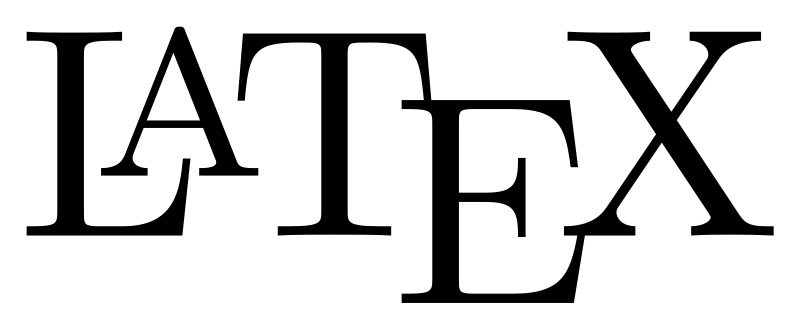
\includegraphics[scale=0.2]{images/latex.png}
\caption{\LaTeX{} Logo}
\end{figure}
\hspace{-1.8em} \LaTeX{}, I had never heard about this term before doing this project,
but when I came to know about it's features, it is just excellent. 
\LaTeX (pronounced /ˈleɪtɛk/, /ˈleɪtɛx/, /ˈlɑːtɛx/, or /ˈlɑːtɛk/) is a 
document markup language and document preparation system for the \TeX{} 
typesetting  program. Within the typesetting system, its name is styled 
as \LaTeX.

\hspace{-1.8em} Within the typesetting system, its name is styled as \LaTeX. The term 
\LaTeX{} refers only to the language in which documents are written, 
not to the editor used to write those documents. In order to create a 
document in \LaTeX, a .tex file must be created using some form of text 
editor. While most text editors can be used to create a \LaTeX{} document, 
a number of editors have been created specifically for working with \LaTeX.\\

\noindent\LaTeX{} is most widely used by mathematicians, scientists, 
engineers, philosophers, linguists, economists and other scholars in 
academia. As a primary or intermediate format, e.g., translating DocBook 
and other XML-based formats to PDF, \LaTeX{} is used because of the 
high quality of typesetting achievable by \TeX. The typesetting system 
offers programmable desktop publishing features and extensive facilities 
for automating most aspects of typesetting and desktop publishing, 
including numbering and cross-referencing, tables and figures, 
page layout and bibliographies.\\

\noindent\LaTeX{} is intended to provide a high-level language that
accesses the power of \TeX. \LaTeX{} essentially comprises a
collection of \TeX{} macros and a program to process \LaTeX documents. 
Because the \TeX{} formatting commands are very low-level, it is usually 
much simpler for end-users to use \LaTeX{}.


\subsubsection{Typesetting}
\LaTeX{} is based on the idea that authors should be able to focus on 
the content of what they are writing without being distracted by its 
visual presentation. in preparing a \LaTeX{} document, the author 
specifies the logical structure using familiar concepts such as 
chapter, section, table, figure, etc., and lets the \LaTeX{} system 
worry about the presentation of these structures. it therefore 
encourages the separation of layout from content while still allowing 
manual typesetting adjustments where needed. 

\begin{verbatim}
\documentclass[12pt]{article}
\usepackage{amsmath}
\title{\LaTeX}
\begin{document}
  \maketitle 
  \LaTeX{} is a document preparation system 
  for the \TeX{} typesetting program.
   \par 
   $E=mc^2$
\end{document}
\end{verbatim}

\subsubsection{Installing \LaTeX{} on System}
Installation of \LaTeX{} on personal system is quite easy. As i have used \LaTeX{} on Ubuntu 13.04 so i am discussing the installation steps for Ubuntu 13.04 here:
\begin{itemize}
\item Go to terminal and type\\\\
\textit{sudo apt-get install texlive-full}
\item Your Latex will be installed on your system and you can check for manual page by typing.\\\\
\textit{man latex}\\

in terminal which gives manual for latex command.
\item To do very next step now one should stick this to mind that the document which one is going to produce is written in any type of editor whether it may be your most common usable editor Gedit or you can use vim by installing first vim into your system using command.\\\\
\textit{sudo apt-get install vim}
\item After you have written your document it is to be embedded with some set of commands that Latex uses so as to give a structure to your document. Note that whenever you wish your document to be looked into some other style just change these set of commands.
\item When you have done all these things save your piece of code with .tex format say test.tex. Go to terminal and type\\\\
\textit{latex path of the file test.tex Or pdflatex path of the file test.tex\\ eg: pdflatex test.tex}\\
for producing pdf file simultaneously.\\
After compiling it type command\\\\
\textit{evince filename.pdf\\ eg: evince test.pdf}\\
To see output pdf file. 
\end{itemize}
\subsubsection{Pdfscreen \LaTeX{}}
There are some packages that can help to have unified document using \LaTeX{}. Example of such a package is pdfscreen that let the user view it’s document in two forms-print and screen. Print for hard copy and screen for viewing your document on screen. Download this package from www.ctan.org/tex-archive/macros/latex/contrib/pdfscreen/.\\
Then install it using above mention method.\\

\noindent To test it the test code is given below:-\\
Just changing print to screen gives an entirely different view. But for working of pdfscreen another package required are comment and fancybox.\\

\noindent The fancybox package provides several different styles of boxes for framing and rotating content in your document. Fancybox provides commands that produce square-cornered boxes with single or double lines, boxes with shadows, and round-cornered boxes with normal or bold lines. You can box mathematics, floats, center, flushleft, and flushright, lists, and pages.\\
 	
\noindent Whereas comments package selectively include/excludes portions of text. The comment package allows you to declare areas of a document to be included or excluded. One need to make these declarations in the preamble of your file. The package uses a method for exclusion that is pretty robust, and can cope with ill-formed bunches of text.\\

\noindent So these extra packages needed to be installed on system for the proper working of pdfscreen package.


	\section{Coding standards of Language used 
}

\subsection{Introduction}
This document is the definition of Google's coding standards for source code in the Java Programming Language. A Java source file is described as being in Google Style if and only if it adheres to the rules herein.
Like other programming style guides, the issues covered span not only aesthetic issues of formatting, but other types of conventions or coding standards as well. However, this document focuses primarily on the hard-and-fast rules that we follow universally, and avoids giving advice that isn't clearly enforceable (whether by human or tool).
\subsection{Source file basics}
\begin{itemize}
\item File name, the source file name consists of the case-sensitive name of the top-level class it contains (of which there is exactly one), plus the .java extension.
\item File encoding: UTF-8 Source files are encoded in UTF-8.Aside from the line terminator sequence, the ASCII horizontal space character (0x20) is the only whitespace character that appears anywhere in a source file. This implies that:
\item All other whitespace characters in string and character literals are escaped.
\item Tab characters are not used for indentation.
\end{itemize}

	\section{GANTT chart
	}
	\begin{figure}[ht]
\centering
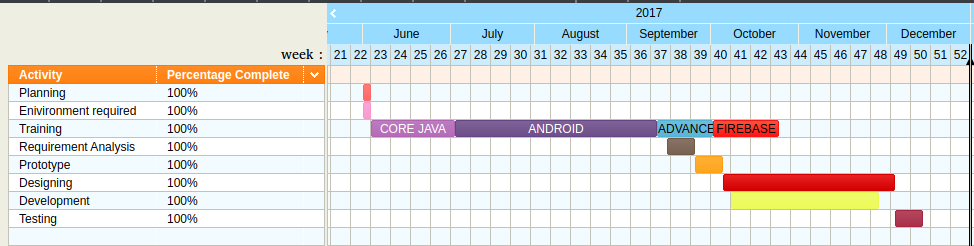
\includegraphics[scale=0.35]{images/ghant.png}
\caption{\LaTeX{} Ghant chart}
\end{figure}
	
	\section{Testing Techniques and Test Plans
}
\subsection{xUnit Framework}
xUnit is the collective name for several unit testing frameworks that derive their structure and functionality from Smalltalk's SUnit. SUnit, designed by Kent Beck in 1998, was written in a highly structured object-oriented style, which lent easily to contemporary languages such as Java and C. Following its introduction in Smalltalk the framework was ported to Java by Kent Beck and Erich Gamma and gained wide popularity, eventually gaining ground in the majority of programming languages in current use. The names of many of these frameworks are a variation on "SUnit", usually replacing the "S" with the first letter (or letters) in the name of their intended language ("JUnit" for Java, "RUnit" for R etc.). These frameworks and their common architecture are collectively known as "xUnit".
\subsection{JUnit}
JUnit is a unit testing framework for the Java programming language. JUnit has been important in the development of test-driven development, and is one of a family of unit testing frameworks which is collectively known as xUnit that originated with SUnit. JUnit is linked as a JAR at compile-time; the framework resides under package junit.framework for JUnit 3.8 and earlier, and under package org.junit for JUnit 4 and later. A research survey performed in 2013 across 10,000 Java projects hosted on GitHub found that JUnit, (in a tie with slf4j-api), was the most commonly included external library. Each library was used by 30.7 percentage of projects.
\subsection{Robotium Android Testing Tool}
Robotium is one the first and frequently utilized automated testing tools for software supported on Android. Robotium is a free Android UI testing tool. It is suitable for tests automation for different Android versions and sub-versions. Software developers often describe it as Selenium for Android. Tests created by Robotium are written in Java. In fact, Robotium is a library for unit tests.
But it takes much time and efforts to create tests by means of Robotium, as one must work with the program source code in order to automate tests. The tool is also unsuitable for interaction with system software; it cannot lock and unlock a smartphone or a tablet. There is no Record and Play function in Robotium, and it does not provide screenshots.
\subsection{MonkeyRunner Android App Testing}
MonkeyRunner Android App Testing
MonkeyRunner is one of popular Android Testing tools used for automating of functional tests for Android software. This tool is more low-level than Robotium is. One does not have to deal with the source code in order to automate tests. The tests are written in Python, one may use a recording tool for creating tests.
MonkeyRunner can run tests on real devices connected to a PC or emulators. The tool has an API what allows it to control a smartphone, a tablet or an emulator from outside of Android code. A significant disadvantage of the mobile app testing tool is that it is necessary to write scripts for each device. Another problem of MonkeyRunner is that the tests require adjustments each time when user interface of the tested program is changed.
\newpage
\subsection{Test Plans}

\subsubsection{Testing of login}

\begin{table}[h!]
\centering
\begin{tabular}{ | m{4.5em} | m{4.5cm}|} 
\hline
Test Id: & TC1   \\ 
\hline
Tester: & Student  \\ 
\hline
Date: & 8-11-2017  \\ 
\hline
Purpose: & Login to system   \\ 
\hline
Pre-requisites: & Must fill login form   \\ 
\hline
Test Data: & Email, Password   \\ 
\hline
Steps: &  \\
\hline  
Step 1 &  Start Application \\ 
Step 2 &  Login Activity will be displayed  \\ 
Step 3 &  Enter password  \\ 
Step 4 &  Click login  \\ 
Step 5 &  If the email and password is correct Home Activity will appear  \\ 
Step 6 &  If the username and password is not correct toast will appear \\
\hline
Status: & Pass   \\ 
\hline
\end{tabular}
\caption{Test Case 1}
\label{table:1}
\end{table}
\newpage
\subsubsection{Testing of Adding News} 	

\begin{table}[h!]
\centering
\begin{tabular}{ | m{5em} | m{5cm}|} 
\hline
Test Id: & TC2   \\ 
\hline
Tester: & Admin  \\ 
\hline
Date: & 12-11-2017  \\ 
\hline
Purpose: & Adding news to database   \\ 
\hline
Pre-requisites: & Must be login   \\ 
\hline
Test Data: & Email, Password, News   \\ 
\hline
Steps: &  \\
\hline  
Step 1 &  Start Application \\ 
Step 2 &  Login Activity will be displayed  \\ 
Step 3 &  Enter password  \\ 
Step 4 &  Click login  \\ 
Step 5 &  Home Activity will appear  \\ 
Step 6 &  Open bottom slider \\
Step 7 &  Click on Add News\\
Step 8 &  Enter valid news(if not added then error display)  \\
Step 9 &  Click on Add News button and it will be uploaded \\
\hline
Status: & Pass   \\ 
\hline
\end{tabular}
\caption{Test Case 2}
\label{table:2}
\end{table}

\newpage
\subsubsection{Testing of retrieving news from database} 	

 \begin{table}[h!]
\centering
\begin{tabular}{ | m{5em} | m{5cm}|} 
\hline
Test Id: & TC3   \\ 
\hline
Tester: & Admin  \\ 
\hline
Date: & 25-11-2017  \\ 
\hline
Purpose: & Retrieving news from database   \\ 
\hline
Pre-requisites: & Must be login and Pdf in database  \\ 
\hline
Test Data: & Email, Password, Any news in database   \\ 
\hline
Steps: &  \\
\hline  
Step 1 &  Start Application \\ 
Step 2 &  Login Activity will be displayed  \\ 
Step 3 &  Enter password  \\ 
Step 4 &  Click login  \\ 
Step 5 & Drag navigation bar and click on latest news \\
Step 5 &  News displayed in Fragment  \\ 
\hline
Status: & Pass   \\ 
\hline
\end{tabular}
\caption{Test Case 3}
\label{table:3}
\end{table}

\newpage
\subsubsection{Testing of adding pdf of athletic meet result} 	

 \begin{table}[h!]
\centering
\begin{tabular}{ | m{5em} | m{5cm}|} 
\hline
Test Id: & TC4   \\ 
\hline
Tester: & Admin  \\ 
\hline
Date: & 25-11-2017  \\ 
\hline
Purpose: & Adding pdf of athletic meet result\\ 
\hline
Pre-requisites: & Must be login and Pdf in mobile memory\\ 
\hline
Test Data: & Email, Password, Pdf    \\ 
\hline
Steps: &  \\
\hline  
Step 1 &  Start Application \\ 
Step 2 &  Login Activity will be displayed  \\ 
Step 3 &  Enter password  \\ 
Step 4 &  Click login  \\ 
Step 5 &  Home Activity will appear  \\ 
Step 6 &  Drag bottom slider and click Add Meet Results button\\
Step 7 &  Enter name of the year and  \\
Step 8 &  Click on SELECT PDF button and select pdf from mobile memory\\
Step 9 &  Click on the Upload Pdf button and Pdf will be uploaded \\ 
\hline
Status: & Pass   \\ 
\hline
\end{tabular}
\caption{Test Case 4}
\label{table:4}
\end{table}

\newpage
\subsubsection{Testing of Map functionality in application} 	

\begin{table}[h!]
\centering
\begin{tabular}{ | m{5em} | m{5cm}|} 
\hline
Test Id: & TC5   \\ 
\hline
Tester: & Student  \\ 
\hline
Date: & 25-11-2017  \\ 
\hline
Purpose: & Checking Map functionality\\ 
\hline
Pre-requisites: & Must be login   \\ 
\hline
Test Data: & Email, Password, Map  \\ 
\hline
Steps: &  \\
\hline  
Step 1 &  Start Application \\ 
Step 2 &  Login Activity will be displayed  \\ 
Step 3 &  Enter password  \\ 
Step 4 &  Click login  \\ 
Step 5 &  Home Activity will appear  \\ 
Step 6 &  Darg right for navigation bar  \\
Step 7 &  Click Map button  \\
Step 8 &  Map of sports department will be apper in the browser\\

\hline
Status: & Pass   \\ 
\hline
\end{tabular}
\caption{Test Case 5}
\label{table:5}
\end{table}

\newpage
\subsubsection{Testing of adding achievement in different categories } 	

 \begin{table}[h!]
\centering
\begin{tabular}{ | m{5em} | m{5cm}|} 
\hline
Test Id: & TC6   \\ 
\hline
Tester: & Admin  \\ 
\hline
Date: & 25-11-2017  \\ 
\hline
Purpose: & Adding achievement different categories   \\ 
\hline
Pre-requisites: & Must be login  \\ 
\hline
Test Data: & Email, Password, content to add achievement   \\ 
\hline
Steps: &  \\
\hline  
Step 1 &  Start Application \\ 
Step 2 &  Login Activity will be displayed  \\ 
Step 3 &  Enter password  \\ 
Step 4 &  Click login  \\ 
Step 5 &  Home Activity will appear  \\ 
Step 6 &  Drag upward for bottom slider  \\
Step 7 &  Choose category(Intramural or Extramural) to add achievement \\
Step 8 &  Click Choose button to upload picture and add description \\
Step 9 &  Click Upload button and achievement will be uploaded \\
\hline
Status: & Pass   \\ 
\hline
\end{tabular}
\caption{Test Case 6}
\label{table:6}
\end{table}
 
 
 
 



\chapter{Results and Discussions}
\section{User Interface Representation (Of  Respective Project)}

The applications interface is designed using custom art elements, the functionality is implemented using Visual studio, and the phase of testing the product was accomplished successfully. The application can very well manage and store the achievement of the students.
Also students can access the latest news published by the department. Athelets are also acknowledge by our automated application.
  



\subsection{Snapshots of system}


\begin{figure}[ht]
\centering
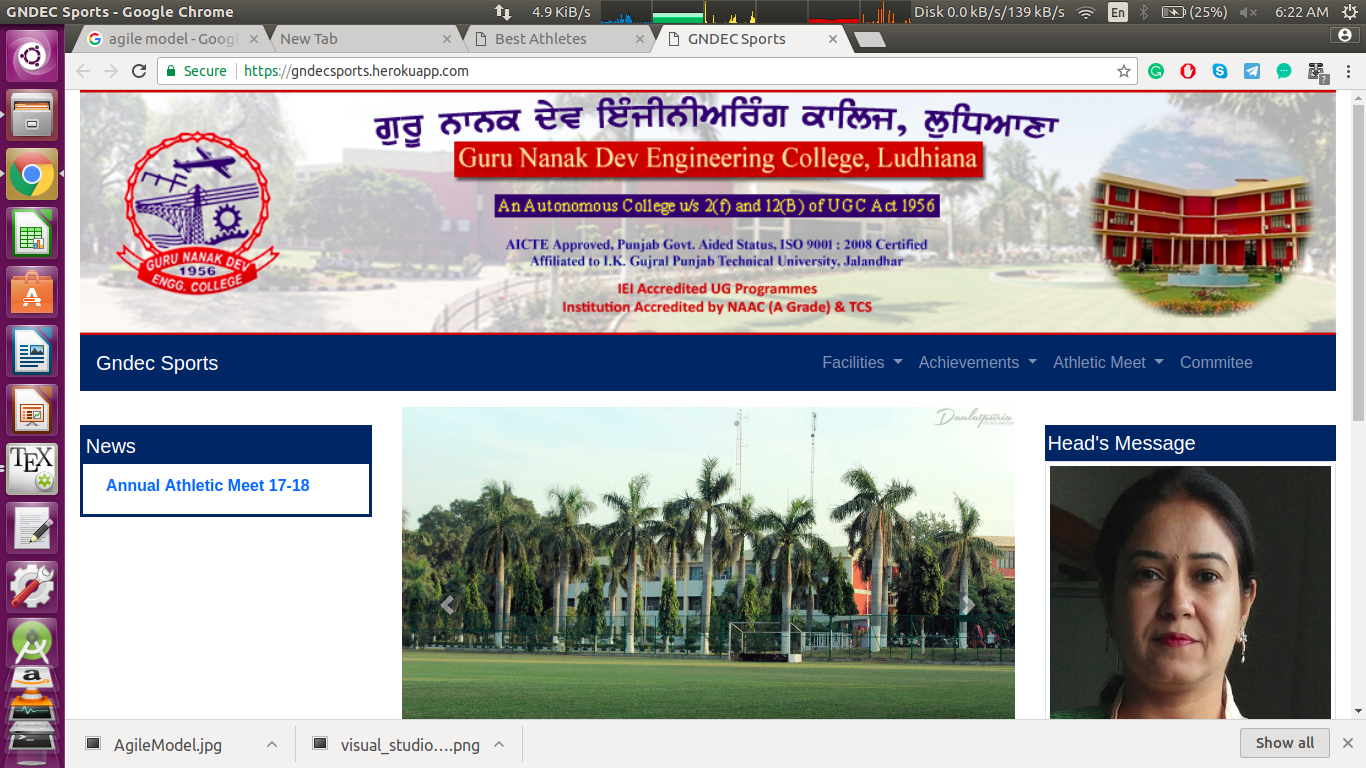
\includegraphics[scale=0.28]{images/HomeUserHeroku.png}
\caption{Home Screen}
\end{figure}

\newpage
\begin{figure}[ht]
\centering
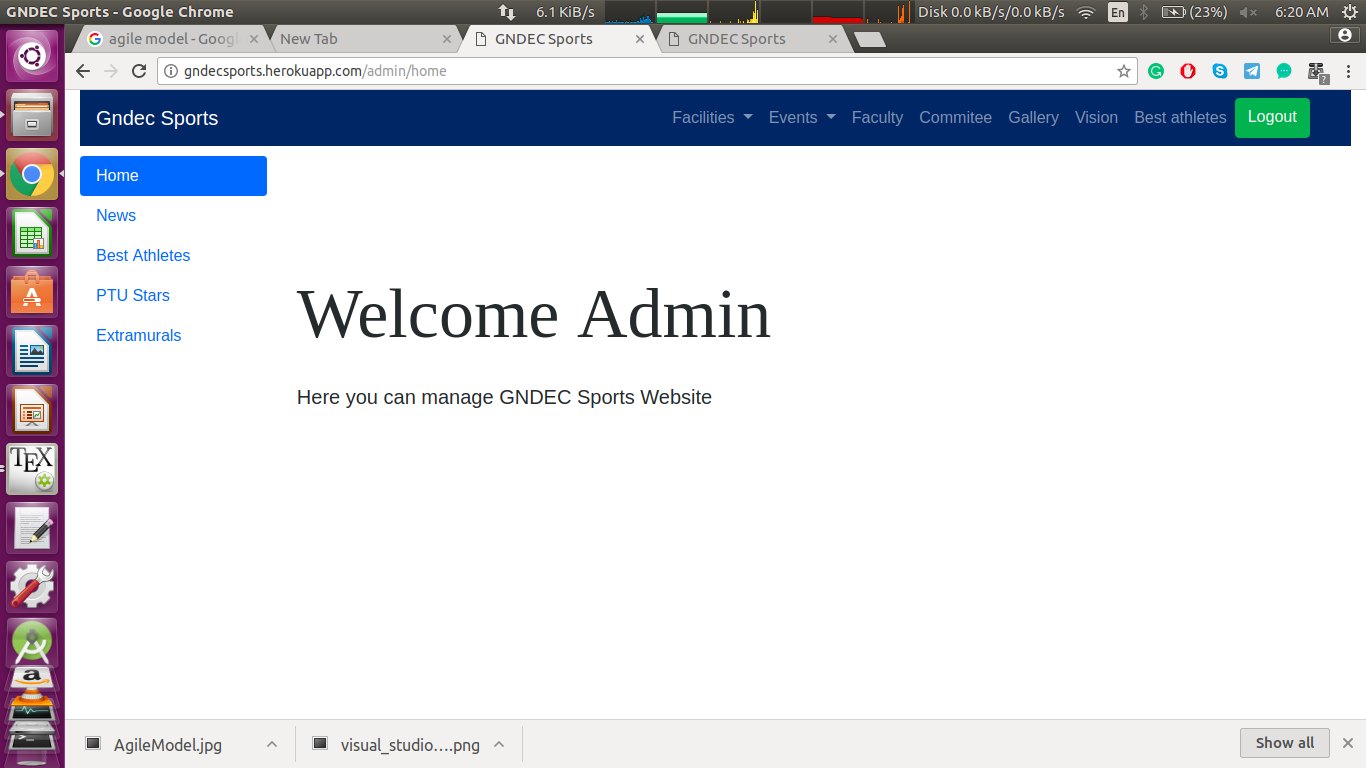
\includegraphics[scale=0.35]{images/HomeAdminHeroku.png}
\caption{Home Screen (Admin)}
\end{figure}

\newpage

\begin{figure}[ht]
\centering
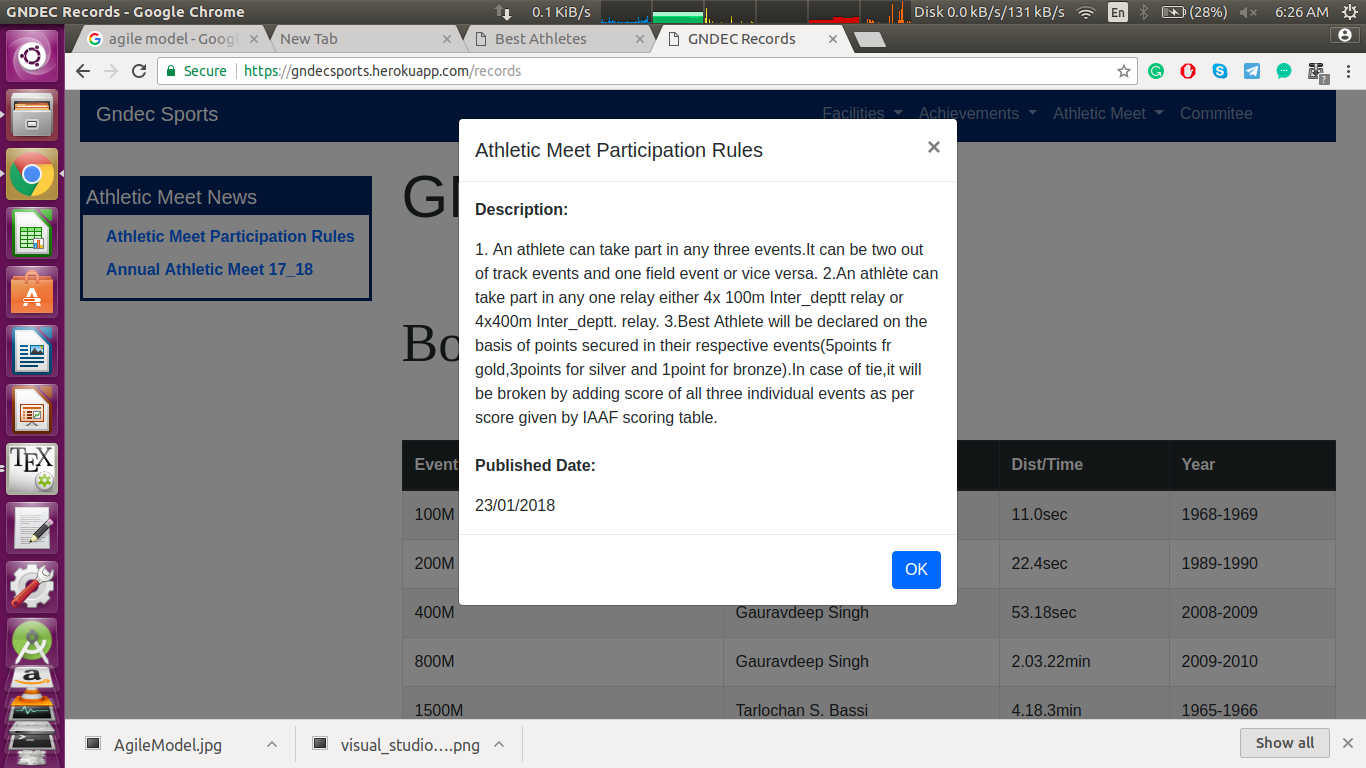
\includegraphics[scale=0.35]{images/NewsPanelHeroku.png}
\caption{News Panel}
\end{figure}

\newpage

\begin{figure}[ht]
\centering
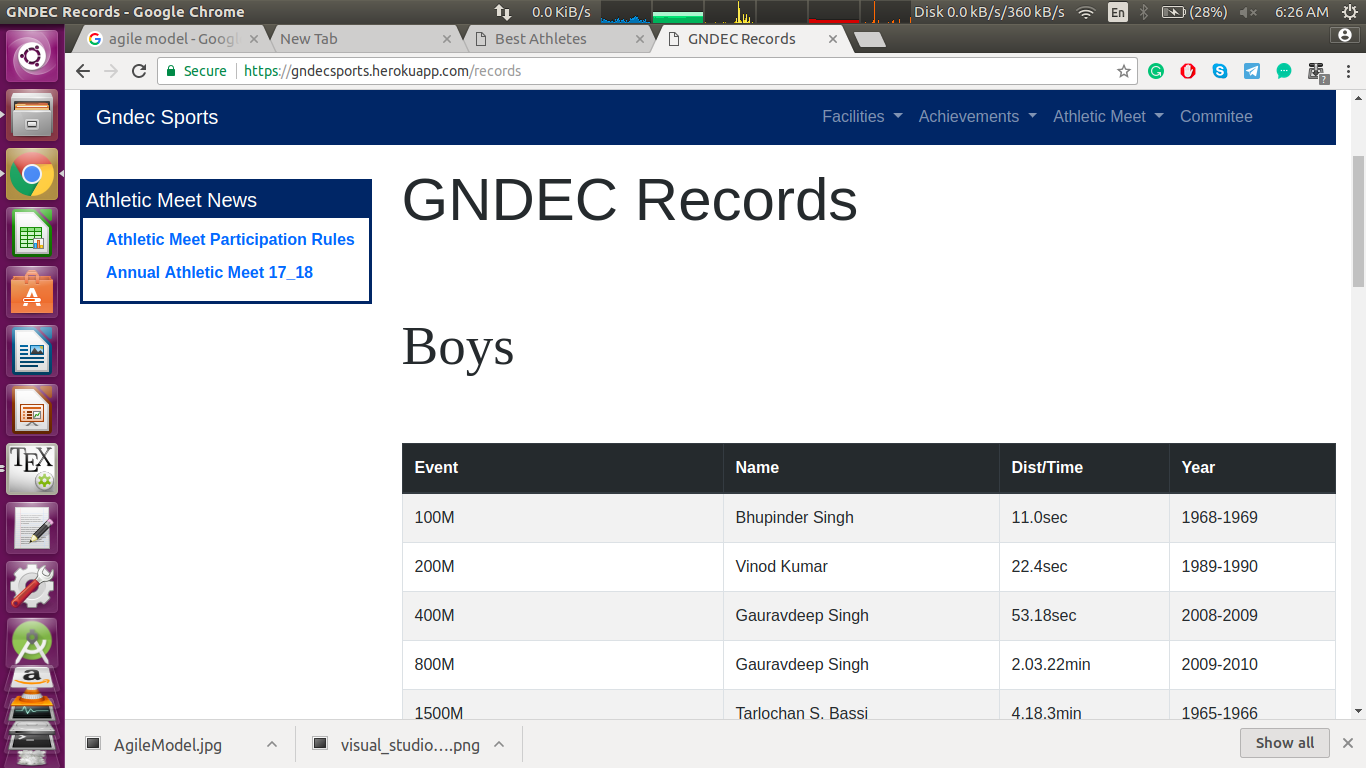
\includegraphics[scale=0.35]{images/RecordsHeroku.png}
\caption{Records}
\end{figure}

\newpage

\begin{figure}[ht]
\centering
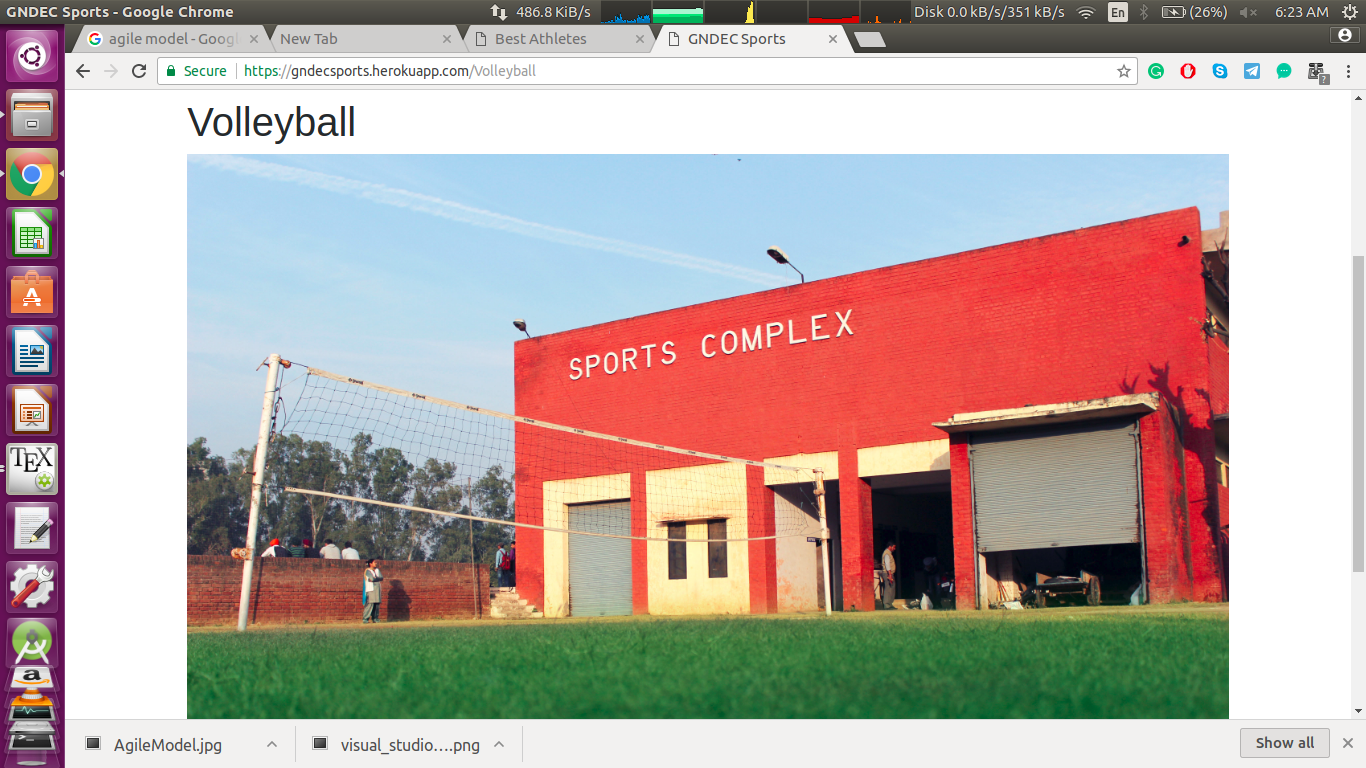
\includegraphics[scale=0.35]{images/VollyballHeroku.png}
\caption{Facilities}
\end{figure}

\newpage

\begin{figure}[ht]
\centering
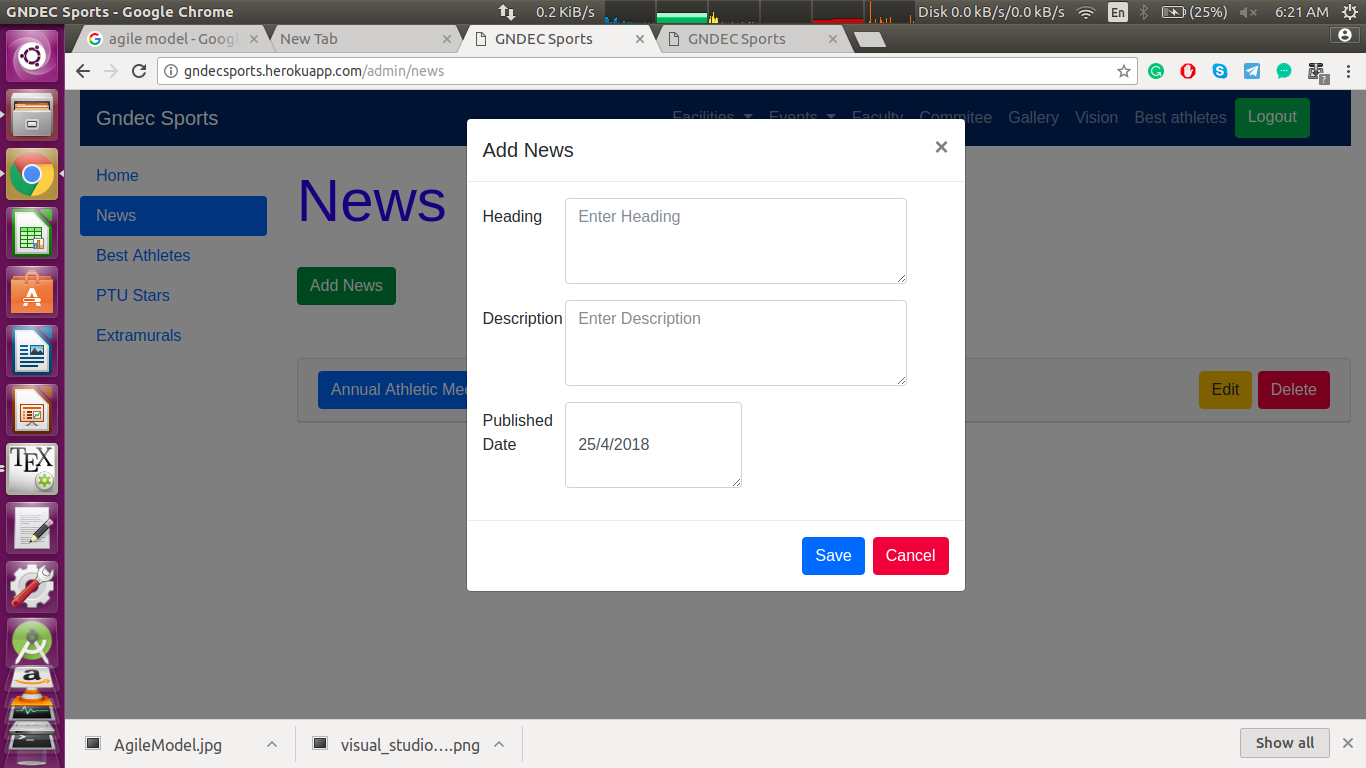
\includegraphics[scale=0.35]{images/AddNewsHeroku.png}
\caption{Add News Panel}
\end{figure}

\newpage

\begin{figure}[ht]
\centering
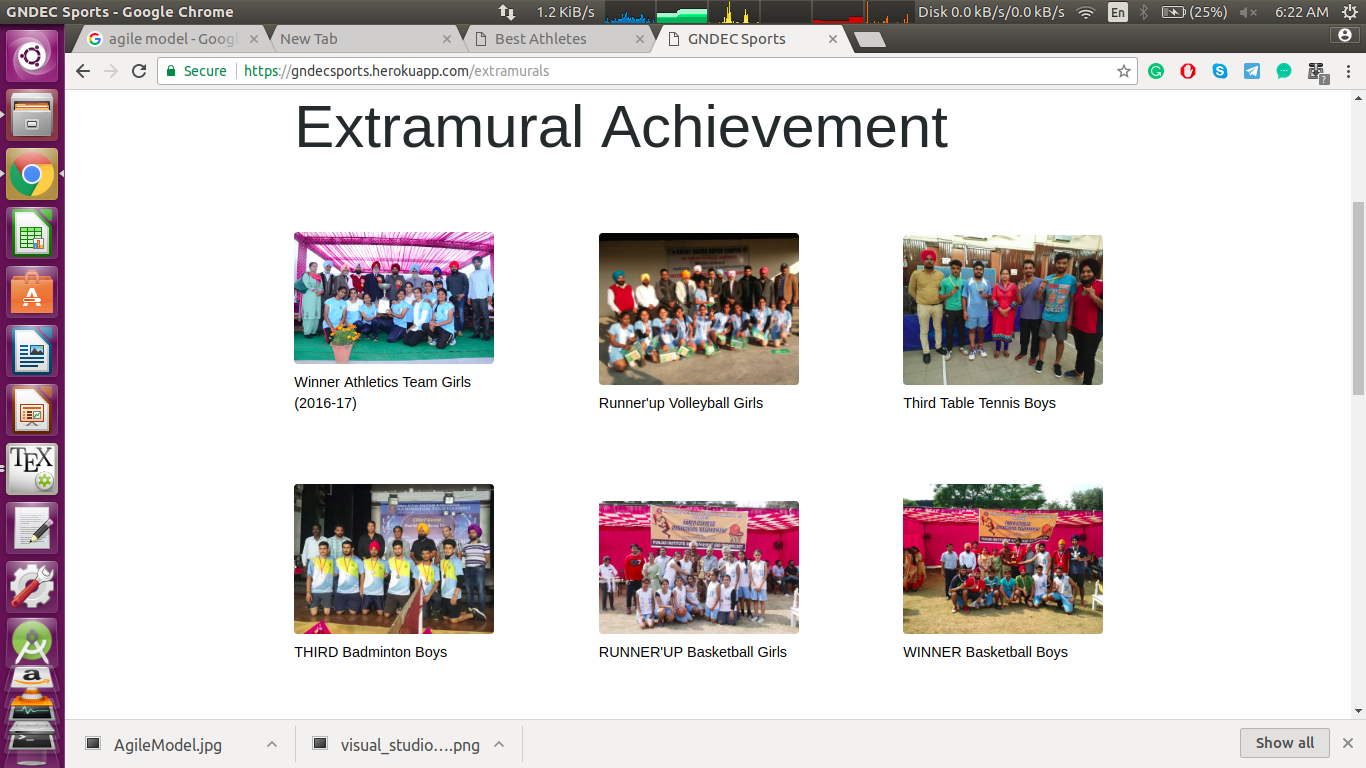
\includegraphics[scale=0.35]{images/AchievementHeroku.png}
\caption{Achievements}
\end{figure}

\newpage

\begin{figure}[ht]
\centering
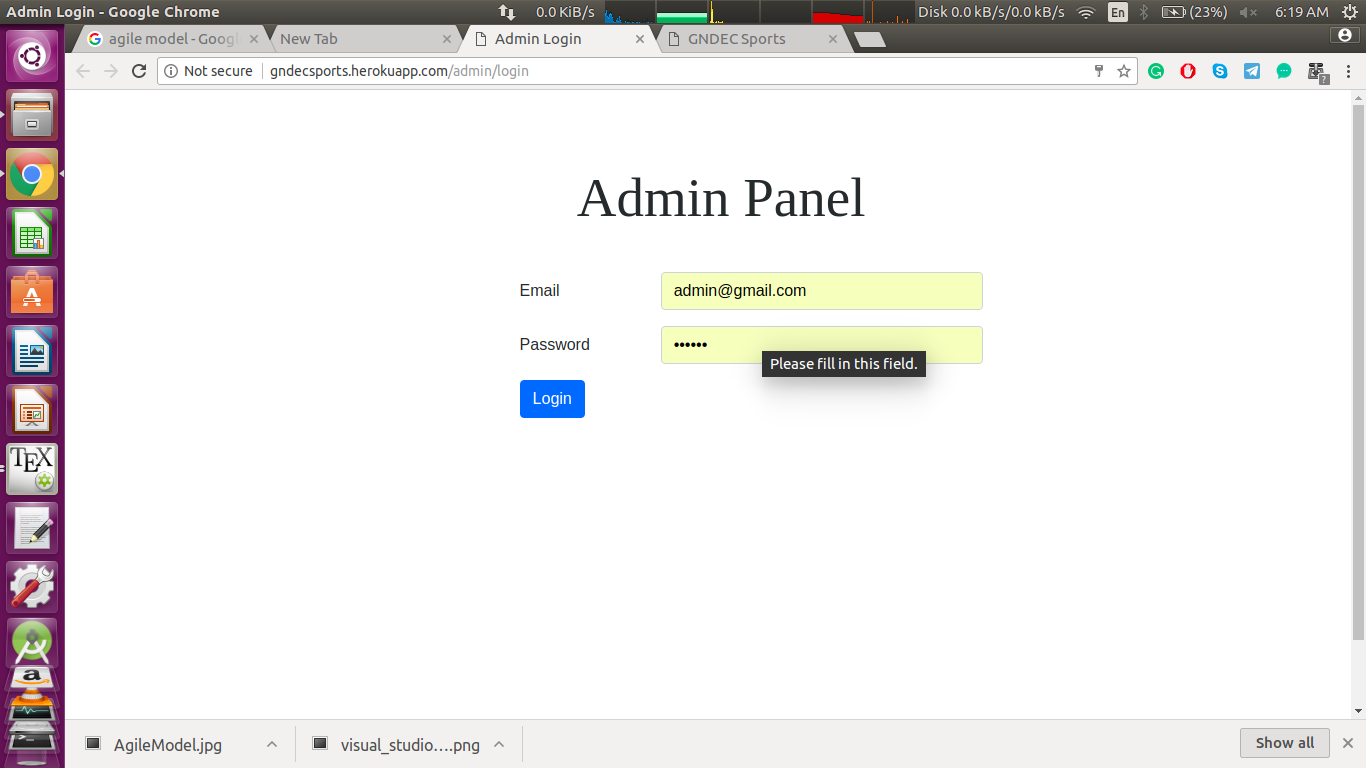
\includegraphics[scale=0.35]{images/AdminPanelHeroku.png}
\caption{Admin Login Panel}
\end{figure}

\newpage

\begin{figure}[ht]
\centering
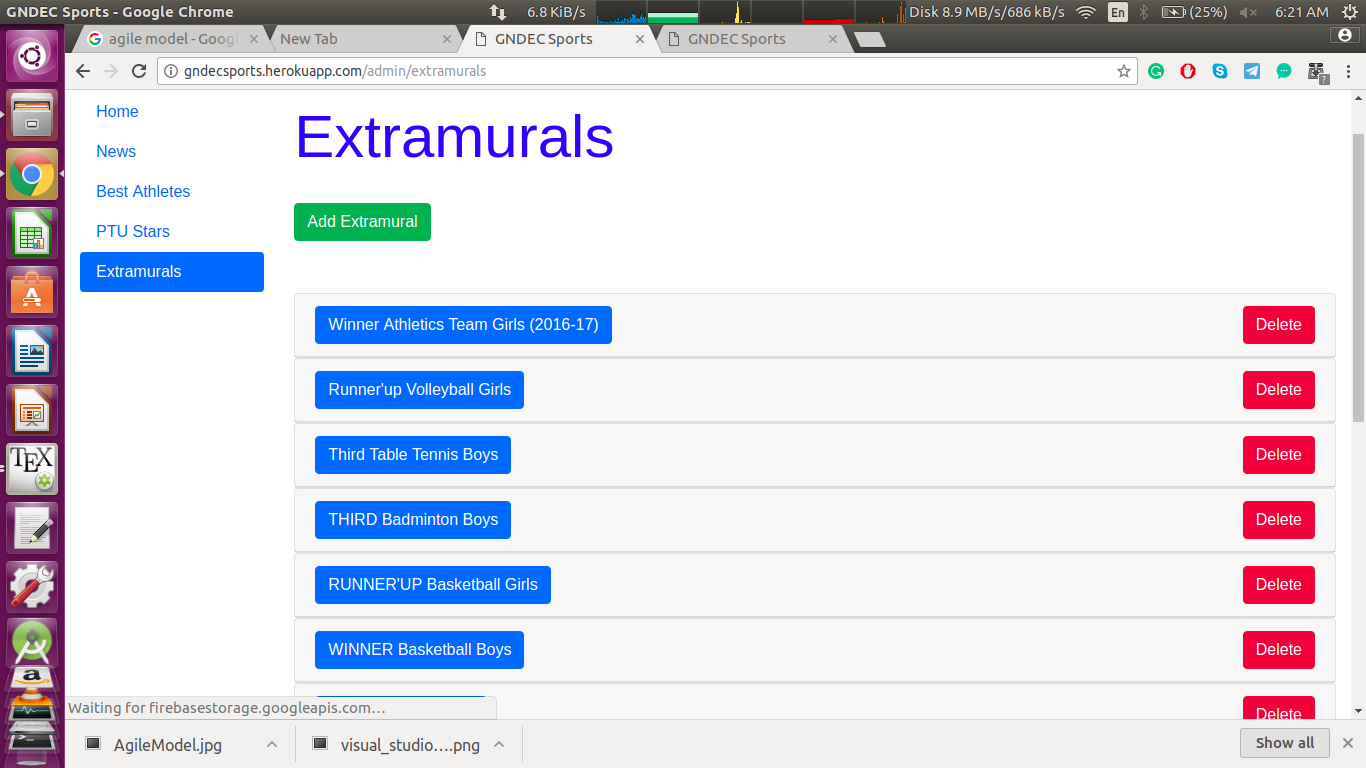
\includegraphics[scale=0.35]{images/ExtramuralHeroku.png}
\caption{Extramural}
\end{figure}


\newpage
\section{Back Ends Representation (Database to be used)}
\subsection{Firebase Realtime Database}
Store and sync data with our NoSQL cloud database. Data is synced across all clients in realtime, and remains available when your app goes offline.

The Firebase Realtime Database is a cloud-hosted database. Data is stored as JSON and synchronized in realtime to every connected client. When you build cross-platform apps with our iOS, Android, and JavaScript SDKs, all of your clients share one Realtime Database instance and automatically receive updates with the newest data.
\subsection{How does it work?}
The Firebase Realtime Database lets you build rich, collaborative applications by allowing secure access to the database directly from client-side code. Data is persisted locally, and even while offline, realtime events continue to fire, giving the end user a responsive experience. When the device regains connection, the Realtime Database synchronizes the local data changes with the remote updates that occurred while the client was offline, merging any conflicts automatically.

The Realtime Database provides a flexible, expression-based rules language, called Firebase Realtime Database Security Rules, to define how your data should be structured and when data can be read from or written to. When integrated with Firebase Authentication, developers can define who has access to what data, and how they can access it.

The Realtime Database is a NoSQL database and as such has different optimizations and functionality compared to a relational database. The Realtime Database API is designed to only allow operations that can be executed quickly. This enables you to build a great realtime experience that can serve millions of users without compromising on responsiveness. Because of this, it is important to think about how users need to access your data and then structure it accordingly.


\newpage
\subsection{Snapshots of Database}
\begin{figure}[ht]
		\centering
		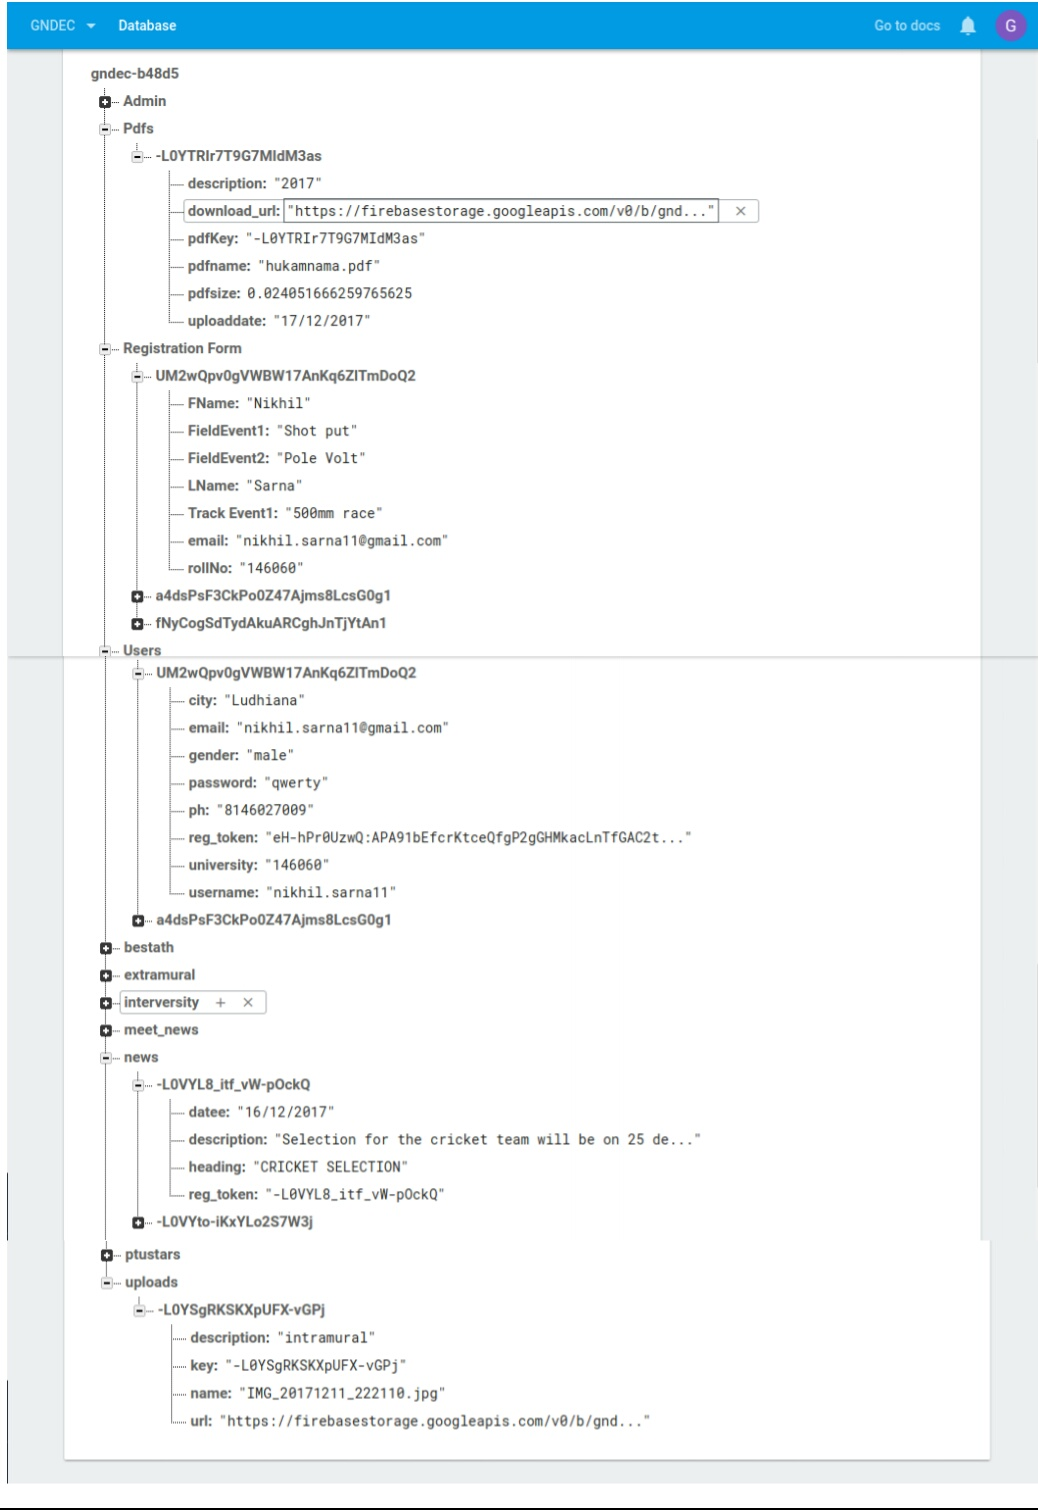
\includegraphics[scale=0.30]{images/dbfire.jpg}
		\caption{Database}
	\end{figure}






\chapter{Conclusion and Future Scope}
\section{Conclusion}
With the coming of \appName, It will encourage sports enthusiasts to take part in the games available in the college. It will become a lot easier for sports commitee to share information or latest news abount the department with the students.Also students will beacme more aware about sports environment available in the college. 

\section{Future Scope}
The app uses android technology which has evergreen scope. The app obviously has a bright
future scope as It will encourage students to participate in the sports.The platform used is
android. Nowadays Android has become very popular which is an open-source, Linux-based
operating system mainly designed by Google for smart-phones and tablets.
Many mobile Apps development industries are considering Android Application Development as one of the best business opportunities, for this they need to hire a lot of knowledgeable
mobile application developer in future. This adds a big sign of scope of mobile Apps in future.
In the current job market of mobile application development, the need for inventive App
developers is huge and still increasing. Android Apps development can also be taken up as
a part time job. You can create your own applications at home and submit it to the Google
Play store which can be downloaded by smart-phone users.
\begin{thebibliography}{3}
\bibitem{} Introduction to Android: http://developer.android.com/guide/index.html
\bibitem{} Android Training: http://developer.android.com/training/index.html.
\bibitem{} Firebase Documentation: https://firebase.google.com/docs/android/setup/
\end{thebibliography}
\end{document}